% Siconos-Doc version 3.0.0, Copyright INRIA 2005-2008.
% Siconos is a program dedicated to modeling, simulation and control
% of non smooth dynamical systems.	
% Siconos is a free software; you can redistribute it and/or modify
% it under the terms of the GNU General Public License as published by
% the Free Software Foundation; either version 2 of the License, or
% (at your option) any later version.
% Siconos is distributed in the hope that it will be useful,
% but WITHOUT ANY WARRANTY; without even the implied warranty of
% MERCHANTABILITY or FITNESS FOR A PARTICULAR PURPOSE.  See the
% GNU General Public License for more details.
%
% You should have received a copy of the GNU General Public License
% along with Siconos; if not, write to the Free Software
% Foundation, Inc., 51 Franklin St, Fifth Floor, Boston, MA  02110-1301  USA
%
% Contact: Vincent ACARY vincent.acary@inrialpes.fr 
%/
\documentclass[10pt]{report}
%$Id: macro.tex,v 1.10 2004/12/08 13:38:58 acary Exp $


%\usepackage{a4wide}
\textheight 25cm
\textwidth 16.5cm
\topmargin -1cm
%\evensidemargin 0cm
\oddsidemargin 0cm
\evensidemargin0cm
\usepackage{layout}


\usepackage{amsmath}
\usepackage{amssymb}
\usepackage{minitoc}
%\usepackage{glosstex}
\usepackage{colortbl}
\usepackage{hhline}
\usepackage{longtable}

%\usepackage{glosstex}
%\def\glossaryname{Glossary of Notation}
\def\listacronymname{Acronyms}

\usepackage[outerbars]{changebar}\setcounter{changebargrey}{20}
%\glxitemorderdefault{acr}{l}

%\usepackage{color}
\usepackage{graphicx,epsfig}
\graphicspath{{figure/}}
\usepackage[T1]{fontenc}
\usepackage{rotating}

%\usepackage{algorithmic}
%\usepackage{algorithm}
\usepackage{ntheorem}
\usepackage{natbib}


%\renewcommand{\baselinestretch}{2.0}
\setcounter{tocdepth}{2}     % Dans la table des matieres
\setcounter{secnumdepth}{3}  % Avec un numero.



\newtheorem{definition}{Definition}
\newtheorem{lemma}{Lemma}
\newtheorem{claim}{Claim}
\newtheorem{remark}{Remark}
\newtheorem{assumption}{Assumption}
\newtheorem{example}{Example}
\newtheorem{conjecture}{Conjecture}
\newtheorem{corollary}{Corollary}
\newtheorem{OP}{OP}
\newtheorem{problem}{Problem}
\newtheorem{theorem}{Theorem}


\newcommand{\CC}{\mbox{\rm $~\vrule height6.6pt width0.5pt depth0.25pt\!\!$C}}
\newcommand{\ZZ}{\mbox{\rm \lower0.3pt\hbox{$\angle\!\!\!$}Z}}
\newcommand{\RR}{\mbox{\rm $I\!\!R$}}
\newcommand{\NN}{\mbox{\rm $I\!\!N$}}

\newcommand{\Mnn}{\mathcal M^{n\times n}}
\newcommand{\Mnp}[2]{\ensuremath{\mathcal M^{#1\times #2}}}



\newcommand{\Frac}[2]{\displaystyle \frac{#1}{#2}}

\newcommand{\DP}[2]{\displaystyle \frac{\partial {#1}}{\partial {#2}}}

% c++ variables writting
\newcommand{\varcpp}[1]{\textit{#1}}
% itemize
\newcommand{\bei}{\begin{itemize}}
\newcommand{\ei}{\end{itemize}}

\newcommand{\ie}{i.e.}
\newcommand{\eg}{e.g.}
\newcommand{\cf}{c.f.}
\newcommand{\putidx}[1]{\index{#1}\textit{#1}}

\def\Er{{\rm I\! R}}
\def\En{{\rm I\! N}} 
\def\Ec{{\rm I\! C}}
 
\def\zc{\hat{z}}
\def\wc{\hat{w}}

\font\tete=cmr8 at 8 pt
\font\titre= cmr12 at 20 pt 
\font\titregras=cmbx12 at 20 pt

%----------------------------------------------------------------------
%                  Modification des subsubsections
%----------------------------------------------------------------------
\makeatletter
\renewcommand\thesubsubsection{\thesubsection.\@alph\c@subsubsection}
\makeatother

%----------------------------------------------------------------------
%             Redaction note environnement
%----------------------------------------------------------------------
\makeatletter
\theoremheaderfont{\scshape}
\theoremstyle{marginbreak}
\theorembodyfont{\upshape}
%\newtheorem{rque}{\bf Remarque}[chapter]
%\newtheorem{rque1}{\bf \fsc{Remarque}}[chapter] !!! \fsc est une commande french
\newtheorem{ndr1}{\textbf{\textsc{Redaction note}}}[section]

\newenvironment{ndr}%
{%
\tt
%\centerline{---oOo---}
\noindent\begin{ndr1}%
}%
{%
\begin{flushright}%
%\vspace{-1.5em}\ding{111}
\end{flushright}%
\end{ndr1}%
%\centerline{---oOo---}
}

\makeatother

%----------------------------------------------------------------------
%             Redaction note environnement V.ACARY
%----------------------------------------------------------------------
\makeatletter
\theoremheaderfont{\scshape}
\theoremstyle{marginbreak}
\theorembodyfont{\upshape}
%\newtheorem{rque}{\bf Remarque}[chapter]
%\newtheorem{rque1}{\bf \fsc{Remarque}}[chapter] !!! \fsc est une commande french
\newtheorem{ndr1va}{\textbf{\textsc{Redaction note V. ACARY}}}[section]

\newenvironment{ndrva}%
{%
\tt
%\centerline{---oOo---}
\noindent\begin{ndr1va}%
}%
{%
\begin{flushright}%
%\vspace{-1.5em}\ding{111}
\end{flushright}%
\end{ndr1va}%
%\centerline{---oOo---}
}

\makeatother
%----------------------------------------------------------------------
%             Redaction note environnement V.ACARY
%----------------------------------------------------------------------
\makeatletter
\theoremheaderfont{\scshape}
\theoremstyle{marginbreak}
\theorembodyfont{\upshape}
%\newtheorem{rque}{\bf Remarque}[chapter]
%\newtheorem{rque1}{\bf \fsc{Remarque}}[chapter] !!! \fsc est une commande french
\newtheorem{ndr1fp}{\textbf{\textsc{Redaction note F. PERIGNON}}}[section]

\newenvironment{ndrfp}%
{%
\tt
%\centerline{---oOo---}
\noindent\begin{ndr1fp}%
}%
{%
\begin{flushright}%
%\vspace{-1.5em}\ding{111}
\end{flushright}%
\end{ndr1fp}%
%\centerline{---oOo---}
}

\makeatother
%----------------------------------------------------------------------
%                  Chapter head enviroment
%----------------------------------------------------------------------
\newenvironment{chapter_head}
{%
\begin{center}%
-------------------- oOo --------------------\\%
\ \\%
\begin{minipage}[]{14cm}%
\noindent\normalsize\advance\baselineskip-1pt %
}%
{%
\par\end{minipage}%
\ \\%
\ \\%
-------------------- oOo --------------------
\end{center}%
\vspace*{\stretch{1}}%
\clearpage%
\thispagestyle{empty}%
\vspace*{\stretch{1}}%
\minitoc%
\vspace*{\stretch{2}}%
\clearpage%
}

%%% Local Variables: 
%%% mode: latex
%%% TeX-master: "report"
%%% End: 

\usepackage{psfrag}
\usepackage{fancyhdr}
\usepackage{subfigure}
%\renewcommand{\baselinestretch}{1.2}
\textheight 23cm
\textwidth 16cm
\topmargin 0cm
%\evensidemargin 0cm
\oddsidemargin 0cm
\evensidemargin 0cm
\usepackage{layout}
\usepackage{mathpple}
\usepackage[T1]{fontenc}
%\usepackage{array}
\makeatletter
\renewcommand\bibsection{\paragraph{References
     \@mkboth{\MakeUppercase{\bibname}}{\MakeUppercase{\bibname}}}}
\makeatother
\usepackage{lastpage}

%% style des entetes et des pieds de page
\fancyhf{} % nettoie le entetes et les pieds
\fancyhead[L]{\texttt{Siconos Development team -- Development Notes }}
\fancyhead[C]{}
\fancyhead[R]{\texttt{\thepage/\pageref{LastPage}}}
\fancyfoot[L]{}
\fancyfoot[C]{}
\fancyfoot[R]{\texttt{file DevNotes.tex -- \isodayandtime}}


\begingroup
\count0=\time \divide\count0by60 % Hour
\count2=\count0 \multiply\count2by-60 \advance\count2by\time
% Min
\def\2#1{\ifnum#1<10 0\fi\the#1}
\xdef\isodayandtime{\the\year-\2\month-\2\day\space\2{\count0}:%
\2{\count2}}
\endgroup




\begin{document}
\thispagestyle{empty}
\title{Developer's Notes}
\author{Siconos Development Team}

\date{\today}
\maketitle

\pagestyle{fancy}
\chapter{First Order Nonlinear Relation }

\begin{table}[!ht]
  \begin{tabular}{|l|l|}
    \hline
    author  & 0. Bonnefon \\
    \hline
    date    & July, 1 2009 \\ 
    \hline
    version & Kernel 3.0.0 \\
    \hline
  \end{tabular}
\end{table}
\chapter{OneStepNSProblem formalisation for several interactions}

\begin{table}[!ht]
  \begin{tabular}{|l|l|}
    \hline
    author  & F. P\'erignon \\
    \hline
    date    & May 16, 2006 \\ 
    \hline
    version & ? \\
    \hline
  \end{tabular}
\end{table}



\section{LinearDS - Linear Time Invariant Relations}
\subsection{General notations}
We consider $n$ dynamical systems of the form:
\begin{equation}
\dot x_i = A_i x_i + R_i 
\end{equation}
Each system if of dimension $n_i$, and we denote $N = \displaystyle{\sum_{i=1}^{n} n_i}$. \\
An interaction, $I_{\alpha}$ is composed with a non smooth law, $nslaw_{\alpha}$ and a relation:
\begin{equation}
y_{\alpha} = C_{\alpha}X_{\alpha} + D_{\alpha}\lambda_{\alpha}
\end{equation}
The ``dimension'' of the interaction, ie the size of vector $y_{\alpha}$, is denoted $m_{\alpha}$ and we set: 
$$ M = \sum_{\alpha=1}^{m} m_{\alpha}$$
$m$ being the number of interactions in the Non Smooth Dynamical System.  \\
$X_{\alpha}$ is a vector that represents the DS concerned by the interaction. Its dimension is noted $N_{\alpha}$, this for $n_{\alpha}$ systems in the interaction. \\
$C_{\alpha}$ is a $m_{\alpha} \times N_{\alpha}$ row-blocks matrix and $D_{\alpha}$ a $m_{\alpha} \times m_{\alpha}$ square matrix. \\
\begin{equation}
C_{\alpha}=\left[\begin{array}{ccc} 
C_{\alpha}^i & C_{\alpha}^j & ...\end{array}\right]
\end{equation}
with $i,j,...\in \mathcal{DS}_{\alpha}$ which is the set of DS belonging to interaction $\alpha$.\\
We also have the following relation: 
\begin{equation}
\left[\begin{array}{c} 
R_{\alpha}^i \\
R_{\alpha}^j \\
...  
\end{array}\right] = B_{\alpha}\lambda_{\alpha}
=\left[\begin{array}{c} 
B_{\alpha}^i \\
B_{\alpha}^j \\
...
\end{array}\right]\lambda_{\alpha}
\end{equation}
$R_{\alpha}^i$ represents the contribution of interaction $\alpha$ on the reaction of the dynamical system $i$, and $B_{\alpha}^i$ is a $n_i \times m_{\alpha}$ block matrix. \\ 
And so: 
\begin{equation}
R_i = \sum_{\beta\in\mathcal{I}_i}R_{\beta}^i=\sum_{\beta\in\mathcal{I}_i}B^i_{\beta} \lambda_{\beta}
\end{equation}
with $\mathcal{I}_i$ the set of interactions in which dynamical system number $i$ is involved. \\
Introducing the time dicretisation, we get: 
\begin{eqnarray}
x_i^{k+1}-x_i^k = h A_i x_i^{k+1} + h R_i^{k+1}  \\
\nonumber\\
y_{\alpha}^{k+1} = C_{\alpha}X_{\alpha}^{k+1} + D_{\alpha}\lambda_{\alpha}^{k+1}\\
\nonumber\\
R_i^{k+1} = \sum_{\beta\in\mathcal{I}_i}B^i_{\beta} \lambda_{\beta}^{k+1}
\end{eqnarray}
ie, with $W_i = (I-h A_i)^{-1}$: 
\begin{eqnarray}
x_i^{k+1}&=& W_i x_i^{k} + hW_i R_i^{k+1}  \\
\nonumber\\
y_{\alpha}^{k+1} &=& C_{\alpha}W_{\alpha} X_{\alpha}^{k} + C_{\alpha}hW_{\alpha}\sum_{\beta\in\mathcal{I}_i}B^i_{\beta} \lambda_{\beta}^{k+1} + D_{\alpha}\lambda_{\alpha}^{k+1} \\
&=& C_{\alpha}W_{\alpha} X_{\alpha}^{k} + (C_{\alpha}hW_{\alpha}B_{\alpha} + D_{\alpha}) \lambda_{\alpha}^{k+1} + \sum_{\beta\neq\alpha}(\sum_{i\in\mathcal{DS}_{\alpha}\cap\in\mathcal{DS}_{\beta}} hC_{\alpha}^iW_i B^i_{\beta} \lambda_{\beta}^{k+1})
\end{eqnarray}
with 
\begin{equation}\label{Walpha}
W_{\alpha}=\left[\begin{array}{ccc} 
W_i &  0   & ... \\
0   &  W_j & ...\\
0  & ... & ... \\ 
\end{array}\right]
\end{equation}
the block-diagonal matrix of all the $W$ for the dynamical systems involved in interaction $\alpha$.\\  
The global-assembled $Y$ vector, of dimension M, composed by $m$ $y_{\alpha}$ subvectors, is given by:
\begin{eqnarray}
Y_{k+1} = q_{OSNSP} + M_{OSNSP}\Lambda_{k+1}
\end{eqnarray}
or,
\begin{eqnarray}
Y_{k+1} =\left[\begin{array}{c} 
y_1 \\
...  \\
y_m
\end{array}\right]_{k+1}
&=&\left[\begin{array}{ccc} 
C_1^1 & \ldots & C_1^n \\
\vdots & \ldots & \vdots \\
C_m^1 & \ldots & C_m^n 
\end{array}\right]\left[\begin{array}{cccc} 
W_1 & 0 & \ldots &0 \\
0  & W_2 & \ddots & \vdots \\
\vdots &\ddots  & \ddots & \vdots \\
&&0& W_n
\end{array}\right]
\left[\begin{array}{c} 
x_1  \\
\vdots \\
\vdots \\
x_n 
\end{array}\right]_k \\
&+&\left[\begin{array}{cccc} 
D_1+h\sum_{j\in \mathcal{DS}_1}C_1^jW_jB_1^j & h\displaystyle{\sum_{j\in \mathcal{DS}_1\cap\mathcal{DS}_2}C_1^jW_jB_2^j} & \ldots &\\
\vdots&\ddots& &\\
& h\displaystyle{\sum_{j\in \mathcal{DS}_m}C_m^jW_jB_{m-1}^j}  & D_m+h\displaystyle{\sum_{j\in \mathcal{DS}_m\cap\mathcal{DS}_{m-1}}C_m^jW_jB_m^j} \\
\end{array}\right]\left[\begin{array}{c} 
\lambda_1  \\
\vdots \\
\lambda_m 
\end{array}\right]_{k+1} \nonumber
\end{eqnarray}
To sum it up, the block-diagonal term of matrix $M_{OSNSP}$, for block-row $\alpha$ is:
\begin{equation}
D_{\alpha}+h\sum_{j\in \mathcal{DS}_{\alpha}}C_{\alpha}^jW_jB_{\alpha}^j
\end{equation}
This is an $m_{\alpha}\times m_{\alpha}$ square matrix.
The extra-diagonal block term, in position ($\alpha,\beta$) is: 
\begin{equation}
h\sum_{j\in \mathcal{DS}_{\alpha}\cap\mathcal{DS}_{\beta}}C_{\alpha}^jW_jB_{\beta}^j
\end{equation}
and is a $m_{\alpha}\times m_{\beta}$ matrix. This matrix differs from 0 when interactions $\alpha$ and $\beta$ are coupled, ie have common DS. \\

Or, for the relation l of interaction $\alpha$, we get: 
\begin{equation}
D_{\alpha,l}+h\sum_{j\in \mathcal{DS}_{\alpha}}C_{\alpha,l}^jW_jB_{\alpha}^j
\end{equation}
for the diagonal, and 
\begin{equation}
h\sum_{j\in \mathcal{DS}_{\alpha}\cap\mathcal{DS}_{\beta}}C_{\alpha,l}^jW_jB_{\beta}^j
\end{equation}
for extra-diagonal terms. \\
$D_{\alpha,l}$, row number $l$ of $D_{\alpha}$, the same for $C_{\alpha,l}$


Finally, the linked-Interaction map provides, for each interaction (named ``current interaction''), the list of all the interactions (named ``linked interaction'') that have common dynamical system with the ``current interaction''.
\subsection{A simple example}

%We consider $n=5$ dynamical systems and $m=4$ interactions: 
%\begin{eqnarray*}
%I_{\mu}& \rightarrow& DS_1, DS_3, m_{\mu} = 3 \\
%I_{\theta}&\rightarrow& DS_3, DS_4, m_{\theta} = 1  \\
%I_{\gamma}&\rightarrow& DS_2,  m_{\gamma} = 1 \\
%I_{\zeta}&\rightarrow& DS_1, DS_5,  m_{\zeta} = 2 
%\end{eqnarray*}
%The linked-interaction map is :
%\begin{eqnarray*}
%I_{\mu} &\rightarrow& I_{\theta}, commonDS = DS_3 \\
%        &\rightarrow& I_{\zeta}, commonDS = DS_1 \\
%I_{\theta} &\rightarrow&I_{\mu}, commonDS = DS_3 \\
%I_{\zeta} &\rightarrow&I_{\mu}, commonDS = DS_1
%\end{eqnarray*}
%And:
%\begin{eqnarray*}
%M &=& 7, N = \displaystyle{\sum_{i=1}^{5} n_i} \\
%\mathcal{I}_1 &=& \{I_{\mu}, I_{\zeta} \}\\
%\mathcal{I}_2 &=& \{I_{\gamma}\} \\
%\mathcal{I}_3 &=& \{I_{\mu}, I_{\theta}\} \\
%\mathcal{I}_4 &=& \{I_{\theta} \} \\
%\mathcal{I}_4 &=& \{I_{\zeta}\}
%\end{eqnarray*}

We consider $n=3$ dynamical systems and $m=2$ interactions: 
\begin{eqnarray*}
I_{\mu}& \rightarrow& \mathcal{DS}_{\mu} = \{DS_1, DS_3\}, m_{\mu} = 3 \\
I_{\theta}&\rightarrow& \mathcal{DS}_{\theta} = \{DS_2, DS_3\}, m_{\theta} = 1  \\
\end{eqnarray*}
The linked-interaction map is :
\begin{eqnarray*}
I_{\mu} &\rightarrow& I_{\theta}, commonDS = DS_3 \\
I_{\theta} &\rightarrow&I_{\mu}, commonDS = DS_3 \\
\end{eqnarray*}
And:
\begin{eqnarray*}
M &=& 4, N = \displaystyle{\sum_{i=1}^{3} n_i} \\
\mathcal{I}_1 &=& \{I_{\mu} \}\\
\mathcal{I}_2 &=& \{I_{\theta}\} \\
\mathcal{I}_3 &=& \{I_{\mu}, I_{\theta}\} \\
\end{eqnarray*}

\begin{eqnarray}
y_1 = \left[\begin{array}{ccc} 
C_1^1 & C_1^3 \end{array}\right]
\left[\begin{array}{c}
x_1 \\
x_3 
\end{array}\right]
+ D_1\lambda_1 \\
y_2 = \left[\begin{array}{ccc} 
C_2^2 & C_2^3 \end{array}\right]
\left[\begin{array}{c}
x_2 \\
x_3 
\end{array}\right]
+ D_2\lambda_2 
\end{eqnarray}
%
\begin{eqnarray}
\left[\begin{array}{c}
R_1 \\
R_2 \\
R_3 \end{array}\right]=
\left[\begin{array}{c}
B_1^1\lambda_1  \\
B_2^2\lambda_2  \\
B_1^3\lambda_1 + B_2^3\lambda_2
\end{array}\right]
\end{eqnarray}
%
\begin{eqnarray}
M_{OSNSP} &=& \left[\begin{array}{cc} 
D_1+hC_1^1W_1B_1^1+hC_1^3W_3B_1^3 & hC_1^3W_3B_2^3 \\
hC_2^3W_3B_1^3 & D_2+hC_2^2W_2B_2^2+hC_2^3W_3B_2^3 
\end{array}\right]\left[\begin{array}{c} 
\lambda_1  \\
\lambda_2
\end{array}\right]_{k+1} 
\end{eqnarray}

\subsection{relative degree}
Let us consider the global vector 
\begin{eqnarray}
Y =\left[\begin{array}{c} 
y_1 \\
...  \\
y_M
\end{array}\right] = CX + D\Lambda
\end{eqnarray}
We denot $r_j$ the relative degree of equation $j$, $j\in [1..M]$. 
We have:
\begin{eqnarray}
y_j = \displaystyle{\sum_{i=1}^n C_j^i x_i +D_{j,j}\lambda_j + \sum_{i\neq j, i=1}^m D_{j,i} \lambda_i } 
\end{eqnarray}
$D_{j,i}$ a scalar and $C_j^i$ a $1 \times n_i$ line-vector. \\
If $D_{jj} \neq 0$, then $r_j=0$. Else, we should consider the first derivative of $y_j$. \\
Before that, recall that: 
\begin{eqnarray}
R_i = \displaystyle{\sum_{k=1}^M B_k^i \lambda_j}
\end{eqnarray}
Through many of the $B_j^i$ are equal to zero, we keep them all in the following lines. \\
Then:

\begin{eqnarray}
\dot y_j &=& \displaystyle{\sum_{i=1}^n C_j^i (A_i x_i +  \sum_{k=1}^M B_k^i \lambda_k  ) + f(\lambda_k)_{k\neq j}} \\
&=& \displaystyle{\sum_{i=1}^n C_j^i (A_i x_i + B_j^i \lambda_j + \sum_{k=1,k\neq j}^M B_k^i \lambda_k  ) + \ldots}
\end{eqnarray}

So, if $\displaystyle{\sum_{i=1}^n C_j^i B_j^i} \neq 0$ (note that this corresponds to the product between line $j$ of $C$ and column $j$ of $B$) 
then $r_j=1$ else we consider the next derivative, and so on.  \\
In derivative $r$, the coefficient of $\lambda_j$ will be:
\begin{eqnarray}
coeff_j&=& \displaystyle{\sum_{i=1}^n C_j^i (A_i)^{r-1} B_j^i }
\end{eqnarray}
if $coeff_j\neq 0$ then $r_j = r$. 

%\subsection{Implementation}
%\begin{itemize}
%\item relative degree: function of $D,C,A$ off all interactions/relations, time invariant $\Rightarrow$ computed and saved in Topology.
%\item linkedInteractionMap $\Rightarrow$ computed and saved in Topology
%\item diagonal term: function of $D,C$ and $B$ of a specific interaction + function of $W$ of all DS concerned + time step. Time invariant.  \\
%$\Rightarrow$ compute and save in OSNSP, during initialize. 
%\item extra-diagonal terms: the same + depends of linkedInteractionMap $\Rightarrow$ compute and save in OSNSP, during initialize.  
%
% ============= LAGRANGIAN =====================
%
\section{LagrangianDS - Lagrangian Linear  Relations}
\subsection{General notations}
We consider $n$ dynamical systems, lagrangian and non linear, of the form: 
\begin{equation}
M_i(q_i) \ddot q_i + N_i(\dot q_i, q_i) = F_{Int,i}(\dot q_i , q_i , t)+F_{Ext,i}(t) + p_i
\end{equation}
Each system if of dimension $n_i$, and we denote $N = \displaystyle{\sum_{i=1}^{n} n_i}$. \\
An interaction, $I_{\alpha}$ is composed with a non smooth law, $nslaw_{\alpha}$ and a relation:
\begin{equation}
y_{\alpha} = H_{\alpha}Q_{\alpha} + b_{\alpha}
\end{equation}
The ``dimension'' of the interaction, ie the size of vector $y_{\alpha}$, is denoted $m_{\alpha}$ and we set: 
$$ M_y = \sum_{\alpha=1}^{m} m_{\alpha}$$
$m$ being the number of interactions in the Non Smooth Dynamical System.  \\
$Q_{\alpha}$ is a vector that represents the DS concerned by the interaction. Its dimension is noted $N_{\alpha}$, this for $n_{\alpha}$ systems in the interaction. \\
$H_{\alpha}$ is a $m_{\alpha} \times N_{\alpha}$ row-blocks matrix and $b_{\alpha}$ a $m_{\alpha}$ vector. \\
\begin{equation}
H_{\alpha}=\left[\begin{array}{ccc} 
H_{\alpha}^i & H_{\alpha}^j & ...\end{array}\right]
\end{equation}
with $i,j,...\in \mathcal{DS}_{\alpha}$ which is the set of DS belonging to interaction $\alpha$.\\
We also have the following relation: 
\begin{equation}
\left[\begin{array}{c} 
R_{\alpha}^i \\
R_{\alpha}^j \\
...  
\end{array}\right] = {}^tH_{\alpha}\lambda_{\alpha}
=\left[\begin{array}{c} 
{}^tH_{\alpha}^i \\
{}^tH_{\alpha}^j \\
...
\end{array}\right]\lambda_{\alpha}
\end{equation}
$R_{\alpha}^i$ represents the contribution of interaction $\alpha$ on the reaction of the dynamical system $i$, and ${}tH_{\alpha}^i$ is a $n_i \times m_{\alpha}$ block matrix. \\ 
And so: 
\begin{equation}
R_i = \sum_{\beta\in\mathcal{I}_i}R_{\beta}^i=\sum_{\beta\in\mathcal{I}_i}{}H^i_{\beta} \lambda_{\beta}
\end{equation}
with $\mathcal{I}_i$ the set of interactions in which dynamical system number $i$ is involved. \\
Introducing the time dicretisation, we get: 
\begin{eqnarray}
\dot q_i^{k+1} = \dot q_{free,i} + W_iR_i^{k+1}
\nonumber\\
\dot y_{\alpha}^{k+1} = H_{\alpha}\dot Q_{\alpha}^{k+1} \\
\nonumber\\
R_i^{k+1} = \sum_{\beta\in\mathcal{I}_i}H^i_{\beta} \lambda_{\beta}^{k+1}
\end{eqnarray}
ie, 
\begin{eqnarray}
  y_{\alpha}^{k+1} &=& H_{\alpha} Q_{\alpha}^{free} + H_{\alpha}W_{\alpha}{}^tH_{\alpha}\lambda_{\alpha}+\sum_{i\in \mathcal{DS}_{\alpha}}\sum_{\beta\in\mathcal{I}_i,\alpha\neq\beta}H_{\alpha}^iW_iH_{\beta}^j\lambda_{\beta}
\end{eqnarray}
with $W_{\alpha}$ given by \eqref{Walpha}. 

The global-assembled $Y$ vector, of dimension M, composed by $m$ $y_{\alpha}$ subvectors, is given by:
\begin{eqnarray}
Y_{k+1} = q_{OSNSP} + M_{OSNSP}\Lambda_{k+1}
\end{eqnarray}

with:
\begin{eqnarray}
q_{OSNSP}^{\alpha} = H_{\alpha} Q_{\alpha}^{free}
\end{eqnarray}
and for $M_{OSNSP}$, the block-diagonal term for block-row $\alpha$ is
\begin{equation}
\sum_{j\in \mathcal{DS}_{\alpha}}H_{\alpha}^jW_j{}^tH_{\alpha}^j
\end{equation}
an $m_{\alpha}\times m_{\alpha}$ square matrix.
The extra-diagonal block term, in position ($\alpha,\beta$) is: 
\begin{equation}
\sum_{j\in \mathcal{DS}_{\alpha}\cap\mathcal{DS}_{\beta}}H_{\alpha}^jW_j{}^tH_{\beta}^j
\end{equation}
and is a $m_{\alpha}\times m_{\beta}$ matrix. This matrix differs from 0 when interactions $\alpha$ and $\beta$ are coupled, ie have common DS. \\

Or, for the relation l of interaction $\alpha$, we get: 
\begin{equation}
\sum_{j\in \mathcal{DS}_{\alpha}}H_{\alpha,l}^jW_j{}^tH_{\alpha}^j
\end{equation}
for the diagonal, and 
\begin{equation}
\sum_{j\in \mathcal{DS}_{\alpha}\cap\mathcal{DS}_{\beta}}H_{\alpha,l}^jW_j{}^tH_{\beta}^j
\end{equation}
for extra-diagonal terms. \\
$H_{\alpha,l}$, row number $l$ of $H_{\alpha}$.


WARNING: depending on linear and non linear case for the DS, there should be a factor h ahead W. See Bouncing Ball template. 

\chapter{Dynamical Systems formulations in Siconos.}

\begin{table}[!ht]
  \begin{tabular}{|l|l|}
    \hline
    author  & F. P\'erignon \\
    \hline
    date    & March 22, 2006 \\ 
    \hline
    version & Kernel 1.1.4 \\
    \hline
  \end{tabular}
\end{table}


\section{Class Diagram}
There are four possible formulation for dynamical systems in Siconos,
two for first order systems and two for second order Lagrangian systems. The main class is DynamicalSystem, all other derived from this one, as shown in the following diagram:
\begin{figure}[htbp]
  \centering
 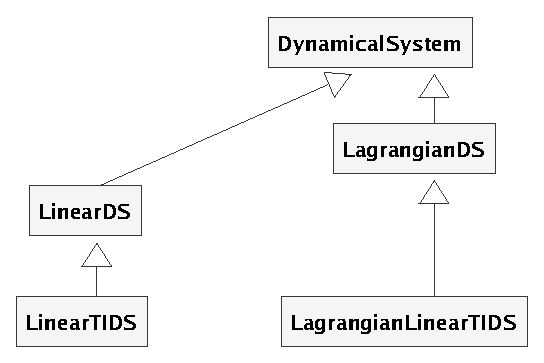
\includegraphics[width=0.3\textwidth]{./DSClassDiagram.eps}
  \label{DSDiagram}
\end{figure}
% DYNAMICAL SYSTEMS
\section{General non linear first order dynamical systems \\ $\rightarrow$ class \it{DynamicalSystem}}
This is the top class for dynamical systems. All other systems classes derived from this one. \\

A general dynamical systems is described by the following set of $n$ equations, completed with initial conditions:
\begin{eqnarray}
  \dot x &=& f(x,t) + T(x) u(x, \dot x, t) + r \\
  x(t_0)&=&x_0 
\end{eqnarray}

\begin{itemize}
\item $x$: state of the system - Vector of size $n$.
\item $f(x,t)$: vector field - Vector of size $n$.
\item $u(x, \dot x, t)$: control term - Vector of size $uSize$.
\item $T(x)$: $n\times uSize$ matrix, related to control term.
\item $r$: input due to non-smooth behavior - Vector of size $n$.
\end{itemize}

The Jacobian matrix, $\nabla_x f(x,t)$, of $f$ according to $x$, $n\times n$ square matrix, is also a member of the class. \\

Initial conditions are given by the member $x_0$, vector of size $n$. This corresponds to x value when
simulation is starting, ie after a call to strategy->initialize(). \\

There are plug-in functions in this class for $f$ (vectorField), $jacobianX$, $u$ and $T$. All
of them can handle a vector of user-defined parameters. 

% LINEAR DS
\section{First order linear dynamical systems $\rightarrow$ class \it{LinearDS}}

Derived from DynamicalSystem, described by the set of $n$ equations and initial conditions: 
\begin{eqnarray}
  \dot x &=& A(t)x(t)+Tu(t)+b(t)+r \\
  x(t_0)&=&x_0 
\end{eqnarray}
With:
\begin{itemize}
\item $A(t)$: $n\times n$ matrix, state independent but possibly time-dependent.
\item $b(t)$: Vector of size $n$, possibly time-dependent.
\end{itemize}
Other variables are those of DynamicalSystem class. \\
$A$ and $B$ have corresponding plug-in functions. \\

Warning: time dependence for $A$ and $b$ is not available at the time in the simulation part for this kind of dynamical systems. \\

Links with vectorField and its Jacobian are: 
\begin{eqnarray}
  f(x,t) &=& A(t)x(t)+b(t) \\
  jacobianX&=&\nabla_x f(x,t) = A(t) 
\end{eqnarray}

% LAGRANGIANDS
\section{Second order non linear Lagrangian dynamical systems \\  $\rightarrow$ class \it{LagrangianDS}}

Lagrangian second order non linear systems are described by the following set of$nDof$ equations + initial conditions:
\begin{eqnarray}
 M(q) \ddot q + NNL(\dot q, q) + F_{Int}(\dot q , q , t) &=& F_{Ext}(t) + p \\
 q(t_0) &=& q0 \\
 \dot q(t_0) &=& velocity0 
\end{eqnarray}
With:
\begin{itemize}
\item $M(q)$: $nDof\times nDof$ matrix of inertia.
\item $q$: state of the system - Vector of size $nDof$.
\item $\dot q$ or $velocity$: derivative of the state according to time - Vector of size $nDof$.
\item $NNL(\dot q, q)$:  non linear terms, time-independent - Vector of size $nDof$.
\item $F_{Int}(\dot q , q , t)$: time-dependent linear terms - Vector of size $nDof$.
\item $F_{Ext}(t)$: external forces, time-dependent BUT do not depend on state - Vector of size $nDof$.
\item $p$: input due to non-smooth behavior - Vector of size $nDof$.
\end{itemize}

The following Jacobian are also member of this class:
\begin{itemize}
\item jacobianQFInt = $\nabla_q F_{Int}(t,q,\dot q)$ - $nDof\times nDof$ matrix.
\item jacobianVelocityFInt = $\nabla_{\dot q} F_{Int}(t,q,\dot q)$ - $nDof\times nDof$ matrix.
\item jacobianQNNL = $\nabla_q NNL(q,\dot q)$ - $nDof\times nDof$ matrix.
\item jacobianVelocityNNL = $\nabla_{\dot q}NNL(q,\dot q)$ - $nDof\times nDof$ matrix.
\end{itemize}


There are plug-in functions in this class for $F_{int}$, $F_{Ext}$, $M$, $NNL$ and the four Jacobian matrices. All
of them can handle a vector of user-defined parameters. \\

Links with first order dynamical system are: 
\begin{eqnarray}
  n &= &2nDof \\
  x &=&\left[\begin{array}{c}q \\ \dot q \end{array}\right] \\
  f(x,t) &=&  \left[\begin{array}{c} \dot q \\ M^{-1}(F_{Ext}-F_{Int}-NNL) \end{array}\right] \\
  \\
  \nabla_x f(x,t) &=& 
  \left[\begin{array}{cc} 
      0_{nDof\times nDof} & I_{nDof\times nDof} \\
      \nabla_q(M^{-1})(F_{Ext}-F_{Int}-NNL) -M^{-1}\nabla_q(F_{Int}+NNL) &  -M^{-1}\nabla_{\dot q}(F_{Int}+NNL) 
    \end{array}\right] \\
  r &=& \left[\begin{array}{c} 0_{nDof} \\ p \end{array}\right] \\
  u(x,\dot x,t) &=& u_L(\dot q, q, t) \text{  (not yet implemented)} \\
  T(x) &=& \left[\begin{array}{c} 0_{nDof} \\ T_L(q) \end{array}\right] \text{  (not yet implemented)} \\
\end{eqnarray}
With $0_{n}$ a vector of zero of size $n$, $0_{n\times m}$ a $n\times m$ zero matrix and
$I_{n\times n}$, identity $n\times n$ matrix. \\

Warning: control terms ($Tu$) are not fully implemented in Lagrangian systems. This will be part of future version.

% LAGRANGIAN LINEAR TIME INVARIANT DS
\section{Second order linear and time-invariant Lagrangian dynamical systems $\rightarrow$ class \it{LagrangianLinearTIDS}}

\begin{eqnarray}
M \ddot q + C \dot q + K q =  F_{Ext}(t) + p
\end{eqnarray}

With:
\begin{itemize}
\item $C$: constant viscosity $nDof\times nDof$ matrix 
\item $K$: constant rigidity $nDof\times nDof$ matrix 
\end{itemize}

And: 
\begin{eqnarray}
F_{Int} &=& C \dot q + K q \\
NNL &=& 0_{nDof} 
\end{eqnarray}



\chapter{Dynamical Systems implementation in Siconos.}

\begin{table}[!ht]
  \begin{tabular}{|l|l|}
    \hline
    author  & F.  P\'erignon \\
    \hline
    date    & November 7, 2006 \\ 
    \hline
    version & Kernel 1.3.0 \\
    \hline
  \end{tabular}
\end{table}




\section{Introduction}
This document is only a sequel of notes and remarks on the way Dynamical Systems are implemented in Siconos.\\
It has to be completed, reviewed, reorganized etc etc for a future Developpers'Guide. \\
See also documentation in Doc/User/DynamicalSystemsInSiconos for a description of various dynamical systems types.

\section{Class Diagram}
There are four possible formulation for dynamical systems in Siconos,
two for first order systems and two for second order Lagrangian systems. The main class is DynamicalSystem, all other derived from this one, as shown in the following diagram:
\begin{figure}[htbp]
  \centering
 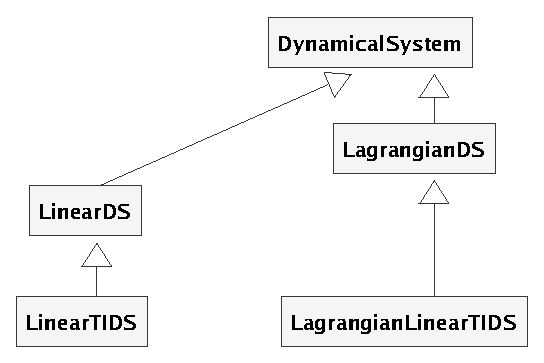
\includegraphics[width=0.3\textwidth]{./DSClassDiagram.eps}
  \label{DSDiagram}
\end{figure}
% DYNAMICAL SYSTEMS

\section{Construction}

Each constructor must:
\begin{itemize}
\item initialize all the members of the class and of the top-class if it exists
\item allocate memory and set value for all required inputs
\item allocate memory and set value for optional input if they are given as argument (in xml for example)
\item check that given data are coherent and that the system is complete (for example, in the LagrangianDS
if the internal forces are given as a plug-in, their Jacobian are also required. If they are not given, this leads to an exception).
\end{itemize}

No memory allocation is made for unused members $\Rightarrow$ requires if statements in simulation.  (if!=NULL ...).\\

\subsection{DynamicalSystem}

\bf{Required data:}\\
n, x0, f, jacobianXF \\
\bf{Optional:}\\
T,u \\

\bf{Always allocated in constructor:} \\
x, x0, xFree, r, rhs, jacobianXF

Warning: default constructor is always private or protected and apart from the others and previous rules or remarks do not always apply to it. 
This for DS class and any of the derived ones. 

\subsection{LagrangianDS}

\bf{Required data:}\\
ndof, q0, velocity0, mass \\
\bf{Optional:}\\
fInt and its Jacobian, fExt, NNL and its Jacobian. \\

\bf{Always allocated in constructor:} \\
mass, q, q0, qFree, velocity, velocity0, velocityFree, p. \\
All other pointers to vectors/matrices are set to NULL by default. \\
Memory vectors are required but allocated during call to initMemory function. 

Various rules:
\begin{itemize}
\item fInt (NNL) given as a plug-in $\Rightarrow$ check that JacobianQ/Velocity are present (matrices or plug-in)
\item any of the four Jacobian present $\Rightarrow$ allocate memory for block-matrix jacobianX  (connectToDS function)
\item 
\end{itemize}

check: end of constructor or in initialize? \\
computeF and JacobianF + corresponding set functions: virtual or not? \\


\section{Specific flags or members}

\begin{itemize}
\item isAllocatedIn: to check inside-class memory allocation
\item isPlugin: to check if operators are computed with plug-in or just directly set as a matrix or vector
\item workMatrix: used to save some specific matrices in order to avoid recomputation if possible (inverse of mass ...)
\end{itemize}

\section{plug-in management}
DynamicalSystem class has a member named parameterList which is a $map<string, SimpleVector*>$, ie a list of
pointers to SimpleVector*, with a string as a key to identified them. 
For example, $parametersList["mass"]$ is a SimpleVector*, which corresponds to the last argument given in 
mass plug-in function. \\
By default, each parameters vectors must be initialized with a SimpleVector of size 1, as soon as the plug-in is
declared. Moreover, to each vector corresponds a flag in isAllocatedIn map, to check if the corresponding vector has been 
allocated inside the class or not. \\ 
For example, in DynamicalSystem, if $isPlugin["vectorField"]==true$, then, during call to constructor or set function,
it is necessary to defined the corresponding parameter: \\
$parametersList["vectorField"] = new SimpleVector(1)$ \\
and to complete the $isAllocatedIn$ flag: \\
$isAllocatedIn["parameter_for_vectorField"] = true$. \\

\chapter{Interactions}
\begin{table}[!ht]
  \begin{tabular}{|l|l|}
    \hline
    author  & F.  P\'erignon \\
    \hline
    date    & November 7, 2006 \\ 
    \hline
    version & Kernel 1.3.0 \\
    \hline
  \end{tabular}
\end{table}

\section{Introduction}
This document is only a sequel of notes and remarks on the way Interactions are implemented in Siconos.\\
It has to be completed, reviewed, reorganized etc etc for a future Developpers'Guide. \\
See also documentation in Doc/User/Interaction.

\section{Class Diagram}

\section{Description}

\begin{ndrfp} 
review of interactions (for EventDriven implementation) 17th May 2006.
\end{ndrfp}

\bei
\item variable \varcpp{nInter} renamed in \varcpp{interactionSize}: represents the size of \varcpp{y} and \varcpp{$\lambda$}. NOT the number of relations !! \\
\item add a variable \varcpp{nsLawSize} that depends on the non-smooth law type.\\
Examples:
\bei
\item NewtonImpact -> \varcpp{nsLawSize} = 1
\item Friction 2D  -> \varcpp{nsLawSize} = 2
\item Friction 3D  -> \varcpp{nsLawSize} = 3
\item ... 
\item \varcpp{nsLawSize} = n with n dim of matrix D in :
$y=Cx+D\lambda$, D supposed to be a full-ranked matrix. \\
Warning: this case is represented by only one relation of size n. 
\ei
\item \varcpp{numberOfRelations}: number of relations in the interaction, \varcpp{numberOfRelations} = $\Frac{\varcpp{interactionSize}}{\varcpp{nsLawSize}}$.
\ei


\chapter{Notes on the Non Smooth Dynamical System construction}
\begin{table}[!ht]
  \begin{tabular}{|l|l|}
    \hline
    author  & F.  P\'erignon \\
    \hline
    date    & November 7, 2006 \\ 
    \hline
    version & Kernel 1.3.0 \\
    \hline
  \end{tabular}
\end{table}

\section{Introduction}

\section{Class Diagram}

\section{Description}

Objects must be constructed in the following order: 
\bei
\item DynamicalSystems
\item NonSmoothLaw: depends on nothing
\item Relation: no link with an interaction during construction, this will be done during initialization. 
\item Interaction: default constructor is private and copy is forbidden. Two constructors: xml and from data. Required data are a DSSet, a NonSmoothLaw and
a Relation (+ dim of the Interaction and a number). \\
Interaction has an initialize function which allocates memory for y and lambda, links correctly the relation and initializes it .... This function is called at the 
end of the constructor. That may be better to call it in simulation->initialize? Pb: xml constructor needs memory allocation for y and lambda if they are
provided in the input xml file. 
\item NonSmoothDynamicalSystem: default is private, copy fobidden. Two constructors: xml and from data. Required data are the DSSet and the InteractionsSet.
The topology is declared and constructed (but empty) during constructor call of the nsds, but initialize in the Simulation, this because it can not be initialize until the nsds has been fully described (ie this to allow user to add DS, Inter ...) at any time in the model, but before simulation initialization). 

\ei

\section{misc}

\bei 
\item no need to keep a number for Interactions? Only used in xml for OSI, to know which Interactions it holds.
\item pb: the number of saved derivatives for y and lambda in Interactions is set to 2. This must depends on the relative degree which is computes during
Simulation initialize and thus too late. It is so not available when memory is allocated (Interaction construction). Problem-> to be reviewed.
\ei 


\chapter{OneStepIntegrator and derived classes.}
\begin{table}[!ht]
  \begin{tabular}{|l|l|}
    \hline
    author  & F.  P\'erignon \\
    \hline
    date    & November 7, 2006 \\ 
    \hline
    version & Kernel 1.3.0 \\
    \hline
  \end{tabular}
\end{table}

\section{Introduction}
This document is only a sequel of notes and remarks on the way OneStepIntegrators are implemented in Siconos.\\
It has to be completed, reviewed, reorganized etc etc for a future Developpers'Guide. \\
See also documentation in Doc/User/OneStepIntegrator for a description of various OSI.

\section{Class Diagram}

\section{Misc}

OSI review for consistency between Lsodar and Moreau:
\begin{itemize}
\item add set of DynamicalSystem*
\item add set of Interaction* 
\item add link to strategy that owns the OSI
\item remove td object in OSI -> future: replace it by a set of td (one per ds)
\item add strat in constructors arg list
\end{itemize}


osi -> strat -> Model -> nsds -> topology \\
osi -> strat -> timeDiscretisation \\

let a timeDiscretisation object in the OSI? set of td (one per ds)? \\
create a class of object that corresponds to DS on the simulation side ? \\
will contain the DS, its discretization, theta for Moreau ... ? \\ 
Allow setStrategyPtr operation? Warning: need reinitialisation. \\


Required input by user: \\
\begin{itemize}
\item list of DS or list of Interactions ? 
\item pointer to strategy
\item ...
\end{itemize}

\section{Construction}

Each constructor must:

\begin{itemize}
\item
\end{itemize}

\subsection{Moreau}

Two maps: one for W, and one for theta. To each DS corresponds a theta and a W. \\
Strategy arg in each constructor.

\bf{Required data:}\\

\bf{Optional:}\\

\bf{Always allocated in constructor:} \\

Warning: default constructor is always private or protected and apart from the others and previous rules or remarks do not always apply to it. 

\subsection{Lsodar}

\bf{Required data:}\\

\bf{Optional:}\\

\bf{Always allocated in constructor:} \\

\chapter{Simulation of a Cam Follower System}
{\bf Main Contributors:} {\textit{Mario di Bernardo, Gustavo Osorio, Stefania Santini}}\\
\textit{University of Naples Federico II, Italy.}\\

%\documentclass[10pt]{article}
%\usepackage[pdftex]{graphicx}
%%$Id: macro.tex,v 1.10 2004/12/08 13:38:58 acary Exp $


%\usepackage{a4wide}
\textheight 25cm
\textwidth 16.5cm
\topmargin -1cm
%\evensidemargin 0cm
\oddsidemargin 0cm
\evensidemargin0cm
\usepackage{layout}


\usepackage{amsmath}
\usepackage{amssymb}
\usepackage{minitoc}
%\usepackage{glosstex}
\usepackage{colortbl}
\usepackage{hhline}
\usepackage{longtable}

%\usepackage{glosstex}
%\def\glossaryname{Glossary of Notation}
\def\listacronymname{Acronyms}

\usepackage[outerbars]{changebar}\setcounter{changebargrey}{20}
%\glxitemorderdefault{acr}{l}

%\usepackage{color}
\usepackage{graphicx,epsfig}
\graphicspath{{figure/}}
\usepackage[T1]{fontenc}
\usepackage{rotating}

%\usepackage{algorithmic}
%\usepackage{algorithm}
\usepackage{ntheorem}
\usepackage{natbib}


%\renewcommand{\baselinestretch}{2.0}
\setcounter{tocdepth}{2}     % Dans la table des matieres
\setcounter{secnumdepth}{3}  % Avec un numero.



\newtheorem{definition}{Definition}
\newtheorem{lemma}{Lemma}
\newtheorem{claim}{Claim}
\newtheorem{remark}{Remark}
\newtheorem{assumption}{Assumption}
\newtheorem{example}{Example}
\newtheorem{conjecture}{Conjecture}
\newtheorem{corollary}{Corollary}
\newtheorem{OP}{OP}
\newtheorem{problem}{Problem}
\newtheorem{theorem}{Theorem}


\newcommand{\CC}{\mbox{\rm $~\vrule height6.6pt width0.5pt depth0.25pt\!\!$C}}
\newcommand{\ZZ}{\mbox{\rm \lower0.3pt\hbox{$\angle\!\!\!$}Z}}
\newcommand{\RR}{\mbox{\rm $I\!\!R$}}
\newcommand{\NN}{\mbox{\rm $I\!\!N$}}

\newcommand{\Mnn}{\mathcal M^{n\times n}}
\newcommand{\Mnp}[2]{\ensuremath{\mathcal M^{#1\times #2}}}



\newcommand{\Frac}[2]{\displaystyle \frac{#1}{#2}}

\newcommand{\DP}[2]{\displaystyle \frac{\partial {#1}}{\partial {#2}}}

% c++ variables writting
\newcommand{\varcpp}[1]{\textit{#1}}
% itemize
\newcommand{\bei}{\begin{itemize}}
\newcommand{\ei}{\end{itemize}}

\newcommand{\ie}{i.e.}
\newcommand{\eg}{e.g.}
\newcommand{\cf}{c.f.}
\newcommand{\putidx}[1]{\index{#1}\textit{#1}}

\def\Er{{\rm I\! R}}
\def\En{{\rm I\! N}} 
\def\Ec{{\rm I\! C}}
 
\def\zc{\hat{z}}
\def\wc{\hat{w}}

\font\tete=cmr8 at 8 pt
\font\titre= cmr12 at 20 pt 
\font\titregras=cmbx12 at 20 pt

%----------------------------------------------------------------------
%                  Modification des subsubsections
%----------------------------------------------------------------------
\makeatletter
\renewcommand\thesubsubsection{\thesubsection.\@alph\c@subsubsection}
\makeatother

%----------------------------------------------------------------------
%             Redaction note environnement
%----------------------------------------------------------------------
\makeatletter
\theoremheaderfont{\scshape}
\theoremstyle{marginbreak}
\theorembodyfont{\upshape}
%\newtheorem{rque}{\bf Remarque}[chapter]
%\newtheorem{rque1}{\bf \fsc{Remarque}}[chapter] !!! \fsc est une commande french
\newtheorem{ndr1}{\textbf{\textsc{Redaction note}}}[section]

\newenvironment{ndr}%
{%
\tt
%\centerline{---oOo---}
\noindent\begin{ndr1}%
}%
{%
\begin{flushright}%
%\vspace{-1.5em}\ding{111}
\end{flushright}%
\end{ndr1}%
%\centerline{---oOo---}
}

\makeatother

%----------------------------------------------------------------------
%             Redaction note environnement V.ACARY
%----------------------------------------------------------------------
\makeatletter
\theoremheaderfont{\scshape}
\theoremstyle{marginbreak}
\theorembodyfont{\upshape}
%\newtheorem{rque}{\bf Remarque}[chapter]
%\newtheorem{rque1}{\bf \fsc{Remarque}}[chapter] !!! \fsc est une commande french
\newtheorem{ndr1va}{\textbf{\textsc{Redaction note V. ACARY}}}[section]

\newenvironment{ndrva}%
{%
\tt
%\centerline{---oOo---}
\noindent\begin{ndr1va}%
}%
{%
\begin{flushright}%
%\vspace{-1.5em}\ding{111}
\end{flushright}%
\end{ndr1va}%
%\centerline{---oOo---}
}

\makeatother
%----------------------------------------------------------------------
%             Redaction note environnement V.ACARY
%----------------------------------------------------------------------
\makeatletter
\theoremheaderfont{\scshape}
\theoremstyle{marginbreak}
\theorembodyfont{\upshape}
%\newtheorem{rque}{\bf Remarque}[chapter]
%\newtheorem{rque1}{\bf \fsc{Remarque}}[chapter] !!! \fsc est une commande french
\newtheorem{ndr1fp}{\textbf{\textsc{Redaction note F. PERIGNON}}}[section]

\newenvironment{ndrfp}%
{%
\tt
%\centerline{---oOo---}
\noindent\begin{ndr1fp}%
}%
{%
\begin{flushright}%
%\vspace{-1.5em}\ding{111}
\end{flushright}%
\end{ndr1fp}%
%\centerline{---oOo---}
}

\makeatother
%----------------------------------------------------------------------
%                  Chapter head enviroment
%----------------------------------------------------------------------
\newenvironment{chapter_head}
{%
\begin{center}%
-------------------- oOo --------------------\\%
\ \\%
\begin{minipage}[]{14cm}%
\noindent\normalsize\advance\baselineskip-1pt %
}%
{%
\par\end{minipage}%
\ \\%
\ \\%
-------------------- oOo --------------------
\end{center}%
\vspace*{\stretch{1}}%
\clearpage%
\thispagestyle{empty}%
\vspace*{\stretch{1}}%
\minitoc%
\vspace*{\stretch{2}}%
\clearpage%
}

%%% Local Variables: 
%%% mode: latex
%%% TeX-master: "report"
%%% End: 

%\usepackage{psfrag}
%\usepackage{fancyhdr}
%\usepackage{subfigure}
%\usepackage{layout}
%\usepackage{mathpple}
%\usepackage{color}
%\usepackage{texdraw} % TeXdraw commands
%\renewcommand{\baselinestretch}{1.2}
%\textheight 23cm \textwidth 16cm \topmargin 0cm \evensidemargin
%0cm \oddsidemargin 0cm \evensidemargin 0cm \makeatletter
%\renewcommand\bibsection{\paragraph{References
%     \@mkboth{\MakeUppercase{\bibname}}{\MakeUppercase{\bibname}}}}
%\makeatother
%%% style des entetes et des pieds de page
%\fancyhf{} % nettoie le entetes et les pieds
%\fancyhead[L]{Template \# 6 : The Case of the Cam-Follower System
%-- G. Osorio, M. di Bernardo, S. Santini.}
%%\fancyhead[C]{V. Acary}%
%\fancyhead[R]{\thepage}
%%\fancyfoot[L]{\resizebox{!}{0.7cm}{\includegraphics[clip]{logoesm2.eps}}}%
%\fancyfoot[C]{}%
%%\fancyfoot[C]{}%
%%\fancyfoot[R]{\resizebox{!}{0.7cm}{\includegraphics[clip]{logo_cnrs_amoi.ps}}}%
%%\addtolength{\textheight}{2cm}
%%\addtolength{\textwidth}{2cm}
%%\pagestyle{empty}
%%\renewcommand{\baselinestretch}{2.0}
%\begin{document}
%%\layout
%\thispagestyle{empty}
%\title{WP6 Template \# 6\\
%The Case of the Cam-Follower System }
%\author{G. Osorio. \hspace{1cm} M. di Bernardo. \hspace{1cm} S. Santini.}
%
%\date{Version 1.0 \\
% \today}
%\maketitle
%
%\pagestyle{fancy}

%\section{Foreword}
%A preliminary analysis will be shown for a simplified model of a
%Cam-Follower system. This system uses lobes (called cams) that
%push against the valves (follower) to open them as the cam
%rotates; springs on the valves return them to their closed
%position. We find that as the rotational speed of the cam varies,
%the valve dynamics can become increasingly complex. From a
%practical viewpoint, it turns out that there is a direct
%relationship between the shape of the cam lobes and the way the
%engine performs in different speed ranges. In particular, the
%shape of the lobes can present sudden changes in the velocity of
%the contact point producing the detachment of the follower with a
%resulting chattering sequence. This is an undesirable behavior
%since the performance of the engine can be seriously affected as
%well as the wear of the components.
%
%In order to perform a suitable simulation of the physical system
%it is necessary to develop numerical routines that can deal with
%several qualitative solutions exhibited by this class of non
%smooth system. Even though this system can be modelled as a
%preloaded forced impact oscillator \cite{bif_chaos2005}, it
%presents several peculiarities that makes worth the study of its
%dynamics. For this work we use the non conservative model that
%presents solutions with chattering sequences and sticking in the
%operational range.
%
%{For the analysis we will show that the unfolding of the complex
%dynamics exhibited by the system under parameter variations can
%only be accounted for by understanding the intricate relationship
%between so-called chattering motion and the occurrence of grazing
%and corner-collision bifurcations. In order to succeed in this
%goal, we make use of recently developed analytical tools for the
%analysis of Non-Smooth Dynamical Systems (NSDS) as bifurcations
%diagrams, phase maps and stroboscopic maps.}
%
%In section 2 we will show the description of the Cam-Follower
%System, in section 3 the numerical strategies including the
%analytical solution with event-driven scheme and the analytical
%tools for NSDS analysis (\ie bifurcation diagrams, phase maps and
%stroboscopic maps.). In section 4 the analysis of the cam-shaft
%dynamical system and finally in section 5 discussion on results
%and future work.
%%\color{blue}\textit{\textbf{Question prof. Mario }}(the effect of
%%having chattering sequence in the rheonomic case
%% (\textit{i.e. when the constrain is time
%%dependant)? (scleronomic vs. rheonomic, conservative vs. non
%%conservative )} \color{black}
%\pagebreak
%\section{Description of the Cam-Follower System}
%\subsection{The cam-follower system as a driven impact oscillator.}
%\textit{\textbf{Bifurcation and chaos in piecewise-smooth
%dynamical systems: Theory and Applications. pg. 15.}\\{DiBernardo,
%Budd, Champneys, Kowalczyk.}}\\
The free body dynamics can be described by a linear second order
system. An external input is considered acting directly on the
follower. This input is a non linear forcing component coming from
the valve. The follower motion is constrained to a phase space
region bounded by the cam position. The non conservative Newton
restitution law is used for the computation of the post impact
velocity. The cam is assumed to be massive therefore only
rotational displacement is allowed. Under these assumptions, the
free body dynamics of the follower can be described by
%equations\ref{eq:sols}
\begin{eqnarray}
  \label{eq:sols}
  \mu\frac{d^2u(t)}{dt^2}+\zeta\frac{du(t)}{dt}+\kappa
  u(t)=f_{v}(t),  \; \text{\hspace{5mm} \text{if} \hspace{3mm}$u(t) > c(t)$.}
\end{eqnarray}
where $\mu$, $\zeta$ and $\kappa$ are constant parameters for the
follower mass, friction viscous damping and spring stiffness
%(restitution constant)
 respectively. The state of the
follower is given by the position $u(t)$ and velocity
$v(t)={\frac{du}{dt}}$. The external forcing is given by $f_v(t)$.
The cam angular position determines $c(t)$ that defines the
holonomic (i.e. constraint only on the position) rheonomic (i.e.
time varying) constraint. The dynamic behavior when impacts occurs
(i.e. $u(t) = c(t)$) is modelled via Newton's impact law that in
this case is given by
\begin{eqnarray}
  \label{eq:il}
  v(t^+)=
  \frac{dc}{dt}-r\left(v(t^-)-\frac{dc}{dt}\right)=(1+r)\frac{dc}{dt}-rv(t^-), \; \text{ \text{if}\hspace{3mm}$
u(t)=c(t)$.}
\end{eqnarray}
where $v(t^+)$ and $v(t^-)$ are the post and pre impact velocities
respectively, $\frac{dc}{dt}$ is the velocity vector of the cam at
the contact point with the follower, and $r \in [0,1]$ is the
restitution coefficient to model from plastic to elastic impacts.
In Figure \ref{Fig:cam-shaft} is presented the schematic diagram
of the physical cam-follower system. In Figure
\ref{Fig:cam-shaft}.a for $t=0$, \ref{Fig:cam-shaft}.b for
$t=\beta$, and \ref{Fig:cam-shaft}.c the profile of the constraint
position $\delta c(t)$, velocity $\frac{dc}{dt}(t)$ and
acceleration $\frac{d^2c}{dt^2}(t)$. It is possible to visualize
the follower displacement as a function of the cam position. It is
also important to notice that different types of cams and
followers profiles are used in practical applications.
\begin{figure}[hbtp]
\setlength{\unitlength}{1mm}
\begin{picture}(90,80)(0,0)
 \put (0,0){\mbox{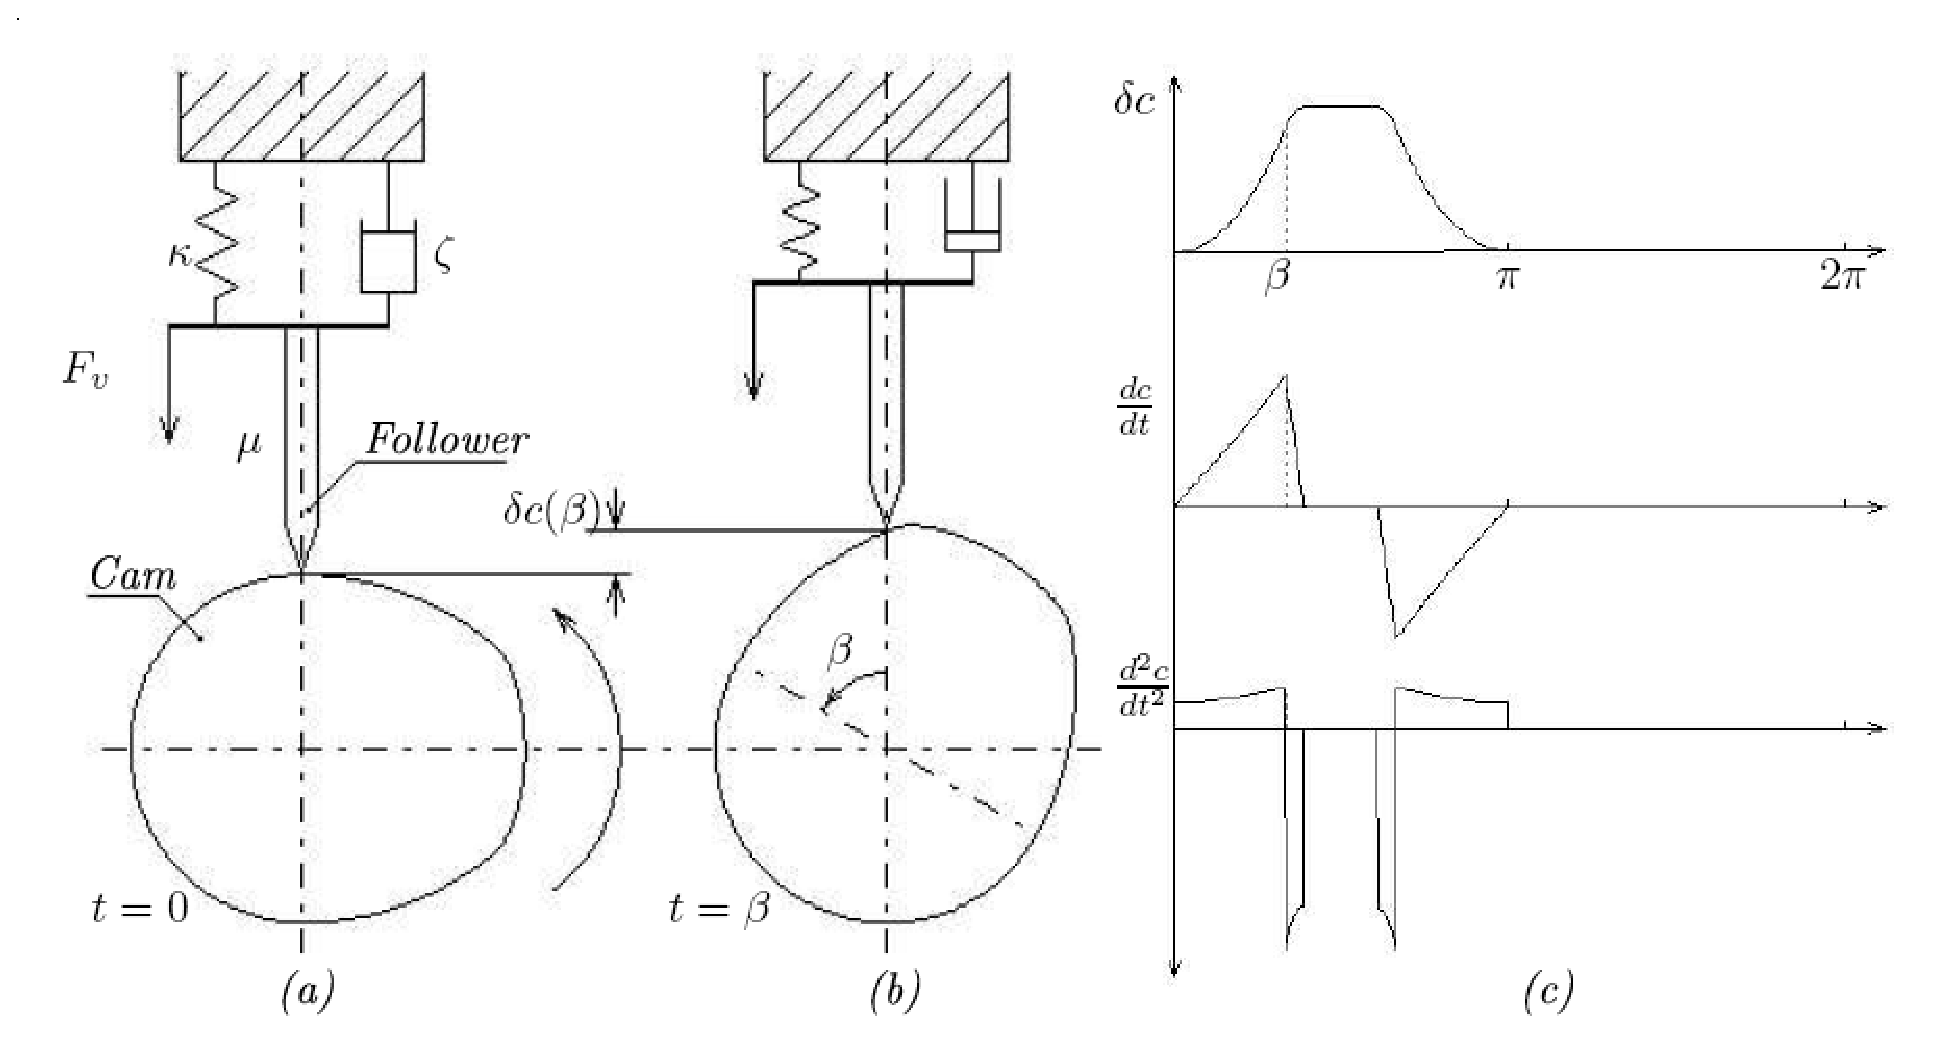
\includegraphics[height=8cm]{./figures/cam}}}
 \put (0,52){\mbox{$F_{v}$}}
 \put (2,34.5){\mbox{\textit{Cam}}}
 \put (26,46){\mbox{\textit{Follower}}}
 \put (15,46){\mbox{\textit{$\mu$}}}
 \put (9,62){\mbox{$\kappa$}}
 \put (32,62){\mbox{$\zeta$}}
 \put (38,40){\mbox{$\delta c (\beta)$}}
 \put (66,28){\mbox{$\beta$}}
 \put (2.5,6){\mbox{\textit{$t=0$}}}
 \put (52.4,6){\mbox{\textit{$t=\beta$}}}
 \put (18.5,-1){\mbox{\textit{(a)}}}
 \put (69.4,-1){\mbox{\textit{(b)}}}
\end{picture}
\begin{picture}(90,80)(-3,0)
 \put (0,0){\mbox{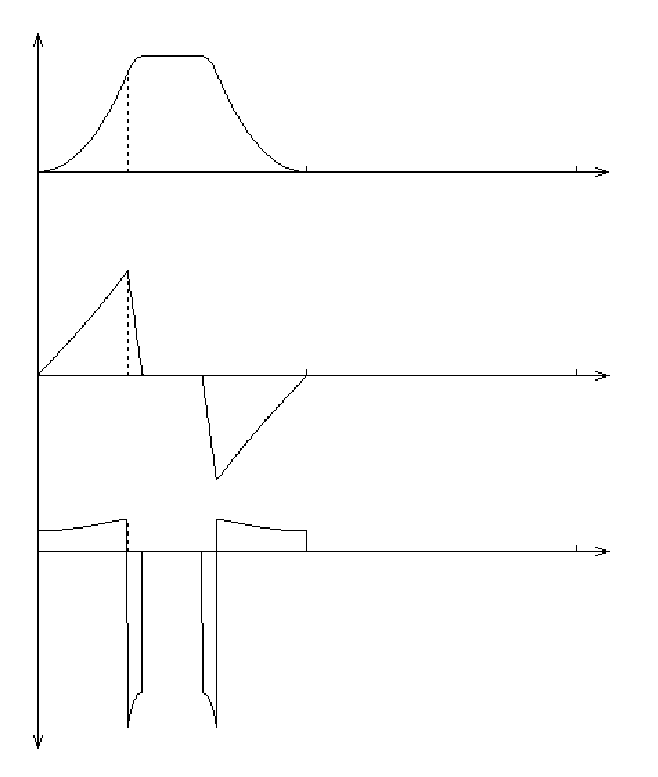
\includegraphics[height=8cm]{./figures/campva}}}
 \put (-3,75){\mbox{$\delta c$}}
 \put (-3,49){\mbox{$ \frac{dc}{dt}$}}
 \put (-3,25){\mbox{$ \frac{d^2c}{dt^2}$}}
 \put (30,60){\mbox{$\pi$}} \put (58,60){\mbox{$2\pi$}}
 \put (10,60){\mbox{$\beta$}}
% \put (30,38){\mbox{$\pi$}} \put (58,38){\mbox{$2\pi$}}
% \put (9,38){\mbox{$\beta$}}
% \put (30,19){\mbox{$\pi$}} \put (58,19){\mbox{$2\pi$}}
% \put (9,19){\mbox{$\beta$}}
 \put (32,-1){\mbox{\textit{(c)}}}
\end{picture}
%\begin{picture}(45,20)(-90,-20)
% \put (3,10){\mbox{$v^{+}=(1+r)\frac{dc}{dt}-rv^{-}$}}
% \put (16,-1){\mbox{\textit{(d)}}}
%\end{picture}
%\begin{picture}(45,20)(-85,-20)
% \put (-2,20){\mbox{$k \hspace{4mm}= \hspace{1.5mm}5 \times 10^{4}\hspace{1.5mm} (N /m)$}}
% \put (-2,16){\mbox{$b \hspace{4mm}= \hspace{1.5mm}0 \hspace{10.5mm}(N\hspace{0.5mm} s/m)$}}
% \put (-2,12){\mbox{$F_{ext} \hspace{0.2mm}= \hspace{1.5mm}0 \hspace{12.5mm}(N)$}}
% \put (-2,8){\mbox{$c \hspace{4mm}\in \hspace{1.5mm}[0.52\hspace{2mm} 0.67]\hspace{2mm}(m)$}}
% \put (-2,4){\mbox{$r \hspace{4mm}= \hspace{1.5mm}0.9$}}
% \put (16,-1){\mbox{\textit{(e)}}}
%\end{picture}
  \caption{Cam-Shaft's schematics. \textit{(a)} t=0. \textit{(b)} t=$\beta$. \textit{(c)} Constraint position $\delta c(t)$, velocity $\frac{dc}{dt}(t)$ and acceleration $\frac{d^{2}c}{dt}(t^{2})$.}
  \label{Fig:cam-shaft}
\end{figure}
\subsection{The cam-follower as a Lagrangian NSDS.}
%\textit{\textbf{WP2 Template 1 Simulation of a bouncing ball with the Moreau's Time-Stepping scheme.}\\{Acary}}\\
 It is possible to completely describe the cam-follower system as a
 driven impact oscillator into the framework of \textit{Lagrangian NSDS} using a
translation in space. Setting $\hat u(t)=u(t)-c(t)$ and $\hat
v(t)= v(t)-dc/dt$, then equations (\ref{eq:sols}) and
(\ref{eq:il}) can be expressed as (the argument $t$ will not be
explicitly written)
\begin{eqnarray}
  \label{eq:trans}
  \mu\frac{d^2\hat u}{dt^2}+\zeta\frac{d\hat u}{dt}+\kappa
  \hat u=f_{v}-\left(\mu\frac{d^2c}{dt^2}+\zeta\frac{dc}{dt}+\kappa
  c\right)&\equiv &\hat f,  \; \text{\hspace{6.5mm} \text{if} \hspace{3mm}$\hat u >
 0$.}\\
\hat v^+&=&-r \hat v^- , \; \text{ \text{if}\hspace{3mm}$\hat
u=0$.}
\end{eqnarray}
Using the framework presented in [2] we have that the equation of
motion of a Lagrangian system may be stated as follows :
\begin{eqnarray}
  \label{eq:lag1}
  M(q)\ddot q + Q(q,\dot q) + F(\dot q, q , t) = F_{ext}(t) + R
\end{eqnarray}

From the (\ref{eq:trans}) we can derive all of the terms which
define a Lagrangian NSDS. In our case the model is completely
linear:
\begin{eqnarray}
  \nonumber
  q&=& \left[\begin{array}{c}  \hat u  \end{array}\right]    \\
  \nonumber
  M(q)&=&  \left[\begin{array}{c} \mu  \end{array}\right] \\
  \label{eq:lag2}
  Q(q,\dot q )& = &\left[\begin{array}{c} 0  \end{array}\right]  \\
  \nonumber
  F(q, \dot q ) &=&  \left[\begin{array}{c} \zeta \end{array}\right] \dot q +  \left[\begin{array}{c} \kappa  \end{array}\right] q\\
  \nonumber
  F_{ext}& = & \left[\begin{array}{c} \hat f \end{array}\right]
\end{eqnarray}

The unilateral constraint requires that:
\begin{eqnarray}
\label{eq:constr} \nonumber
 \hat u \geq 0
\end{eqnarray}
so we can obtain
\begin{eqnarray}
y &= & H^T q + b \\
\nonumber H^T &=&\left[\begin{array}{c} 1 \end{array}\right]\\
\nonumber b&=&0
\end{eqnarray}

In the same way, the reaction force due to the constraint is
written as follows:
\begin{eqnarray}
\nonumber R=H \lambda, \hspace{1cm}  \text{with }
H=\left[\begin{array}{c} 1
\end{array}\right]
\end{eqnarray}

The unilataral contact law may be formulated as follow:
\begin{eqnarray}
  \label{eq:17}
  0 \leq y \perp \lambda\geq 0
\end{eqnarray}
and the Newton's impact law:
\begin{eqnarray}
  \label{eq:17}
\text{If } y=0, \dot{y}^+ =-r\dot{y}^-
\end{eqnarray}

\subsection{Implementation in the platform}
%The code for the simulation of the Cam Follower system using the
%SICONOS software package is:
For the simulation of the cam follower system follow the steps

\begin{enumerate}
\item Move to the working directory \verb"sample/CamFollower"

\verb"$cd sample/CamFollower "

\item Clean the directory form binary files using the
\verb"siconos" command

\verb"$siconos -c "

\item Compile the file \verb"CamFollowerNoXml.cpp" in
the sample folder ({\em See} the code at the end of the section)

\verb"$siconos CamFollowerNoXml.cpp"

\item Change the simulation parameters ({\em i.e.}
Follower initial position and velocity, cam initial angle,
simulations time, cam rotational speed in rpm, etc.) in the file
\verb"CamFollowerNoXml.cpp".

\end{enumerate}

Next we present the sample code for the
\verb"CamFollowerNoXml.cpp" file:
\begin{tabbing}
\hspace{1cm}\= \hspace{0.5cm}\= \hspace{1cm}\= \hspace{1cm}\= \hspace{1cm}\\
 \> \+ int main(int argc, char* argv[]) {\bf \{} \\
 \>  {\bf\{} \+ \hspace{0.5cm}\= \hspace{2cm}\= \hspace{1cm}\=\hspace{1cm}\=\hspace{1cm}\=\hspace{1cm}\=\\
 \> \em   // ======== Creation of the model =============\\
 \> \em  // User-defined main parameters\\

 \> double rpm=358; \\
 \> double phi\_0=0;\\

 \> unsigned int dsNumber = 1; \>\>\>\> \em // the Follower and the ground\\
 \> unsigned int nDof = 1;  \>\>\>\>    \em // degrees of freedom for the Follower\\
 \> double t0 = 0;            \>\>\>\>  \em   // initial computation time\\
 \> double T = 5;             \>\>\>\>  \em    // final computation time\\
 \> double h = 0.0001;   \>\>\>\>       \em // time step\\
 \> int Kplot;\\
 \> Kplot=(int)(Tplot/h);\\

 \> double position\_init = 0.4;\>\>\>\> \em// initial position for lowest bead.\\
 \> double velocity\_init = 0.4;\>\>\>\> \em// initial velocity for lowest bead.\\
 \\
 \> \em    // ======= Dynamical systems =========\\
 \\
 \>     vector<DynamicalSystem *> vectorDS; // the list of DS\\
 \>     vectorDS.resize(dsNumber,NULL);\\
\\
 \> SiconosMatrix *Mass, *K, *C;        // mass/rigidity/viscosity\\
 \> Mass = new SiconosMatrix(nDof,nDof);\\
 \> (*Mass)(0,0) = 1.221;\\
 \> K = new SiconosMatrix(nDof,nDof);\\
 \> (*K)(0,0) = 1430.8;\\
 \> C = new SiconosMatrix(nDof,nDof);\\
 \> (*C)(0,0) = 0;\\
\\
 \>  //  Initial positions and velocities  \\
 \>  vector<SimpleVector *> position\_0;\\
 \>  vector<SimpleVector *> velocity\_0;\\
 \>  position\_0.resize(dsNumber,NULL);\\
 \>  velocity\_0.resize(dsNumber,NULL);\\
 \>  position\_0[0] = new SimpleVector(nDof);\\
 \>  velocity\_0[0] = new SimpleVector(nDof);\\
 \>  (*(position\_0[0]))(0) = position\_init;\\
 \>  (*(velocity\_0[0]))(0) = velocity\_init;\\
 \\
 \>  vectorDS[0] =\\ \>
 new LagrangianLinearTIDS(0,nDof,*(position\_0[0]),*(velocity\_0[0]),*Mass,*K,*C);\\
\\
 \> static\_cast<LagrangianDS*>(vectorDS[0])
 \\ \>\>\>->setComputeFExtFunction("FollowerPlugin.so", "FollowerFExt");\\
\\
 \> // Example to set a list of parameters in FExt function.\\
 \> // 1 - Create a simple vector that contains the required
 parameters.\\
\\
 \> // Here we set two parameters, the DS  number.\\
 \> SimpleVector * param = new SimpleVector(2);\\
\\
 \> (*param)(0)=rpm;\\
 \> (*param)(1)=phi\_0;\\
 \> // 2 - Assign this param to the function FExt\\
 \> static\_cast<LagrangianDS*>(vectorDS[0])->setParametersListPtr(param,2);\\
 \> // 2 corresponds to the position of FExt in the stl vector of possible parameters. \\
\> //  0 is mass, 1 FInt.\\ % and so on.\\
 \> // Now the cam rotational velocity in rpms will be available in FExt plugin.\\
\\
\> // ===== Interactions =====\\
\\
 \>  vector<Interaction*> interactionVector;\\
 \>  interactionVector.resize(1,NULL);\\
 \>  vector<DynamicalSystem*> *dsConcerned = \\ \>\>\> new vector<DynamicalSystem*>(dsNumber);\\
\\
 \>  // ===== Non Smooth Law =====\\
 \>  double e = 0.8;\\

 \>  // Interaction Follower-floor\\
 \>  SiconosMatrix *H = new SiconosMatrix(1,nDof);\\
 \>  (*H)(0,0) = 1.0;\\
 \>  NonSmoothLaw * nslaw = new NewtonImpactLawNSL(e);\\
 \>  Relation * relation = new LagrangianLinearR(*H);\\
 \>  (*dsConcerned)[0] = vectorDS[0];\\

 \>  interactionVector[0] = new Interaction("Follower-Ground",0,1, dsConcerned);\\
 \>  interactionVector[0]->setRelationPtr(relation);\\
 \>  interactionVector[0]->setNonSmoothLawPtr(nslaw);\\

 \> // ===== Interactions =====\\
\\
 \> // ===== NonSmoothDynamicalSystem =====\\

 \> bool isBVP =0;\\
 \> NonSmoothDynamicalSystem * nsds = \\
\>\>\>\> new NonSmoothDynamicalSystem(isBVP);\\
\\
 \>// Set DS of this NonSmoothDynamicalSystem\\
 \> nsds->setDynamicalSystems(vectorDS);       \\
 \> // Set interactions of the  NonSmoothDynamicalSystem\\
 \> nsds->setInteractions(interactionVector);  \\
\\
 \> // ===== Model =====\\
\\
 \> Model * Follower = new Model(t0,T);\\
 \> // set NonSmoothDynamicalSystem of this  model\\
 \> Follower->setNonSmoothDynamicalSystemPtr(nsds);\\
 \\
 \> // ====== Strategy ======\\
\\
 \> double theta = 0.5;  \>\>\>      // theta for Moreau integrator\\
 \> string solverName = "QP" ;\\
\\
 \> Strategy* S = new TimeStepping(Follower);\\
\\
 \> // -- Time discretisation --\\
 \> TimeDiscretisation * t = new TimeDiscretisation(h,S);\\
\\
 \> // -- OneStepIntegrators --\\
 \> vector<OneStepIntegrator *> vOSI;\\
 \> vOSI.resize(dsNumber,NULL);\\
 \> vOSI[0] = new Moreau(t,vectorDS[0],theta);\\
 \> S->setOneStepIntegrators(vOSI);\\
\\
 \> // -- OneStepNsProblem --\\
 \> OneStepNSProblem * osnspb = new LCP(S,solverName,101, 0.0001,"max",0.6);\\
 \> S->setOneStepNSProblemPtr(osnspb); // set OneStepNSProblem of the
 strategy\\
 \> cout << "=== End of model loading === " << endl;\\
 \> // ==== End of model definition======\\
\\
\\
\\
 \> // ========= Computation============\\
\\
 \> // --- Strategy initialization ---\\
 \> S->initialize();\\
 \> cout <<"End of strategy initialisation" << endl;\\
\\

 \> int k = t->getK(); \> \> \> \> // Current step\\
 \> int N = t->getNSteps(); \> \> \> \> // Number of time steps\\
\\
 \> // --- Get the values to be plotted ---\\
 \> // -> saved in a matrix dataPlot\\
 \> unsigned int outputSize = 8;\\
\\
 \> SiconosMatrix DataPlot(Kplot+1,outputSize );\\
 \>   // For the initial time step:\\
 \\
 \> // time\\
 \>     DataPlot(k,0) = k*t->getH();\\
 \\
 \>     DataPlot(k,1) = static\_cast<LagrangianDS*>(vectorDS[0])->getQ()(0);\\
 \>     DataPlot(k,2) = static\_cast<LagrangianDS*>(vectorDS[0])->getVelocity()(0);\\
 \>     DataPlot(k,3) = (Follower->getNonSmoothDynamicalSystemPtr()->\\
 \> \> getInteractionPtr(0)->getLambda(1))(0);\\
 \>     DataPlot(k,4) = static\_cast<LagrangianDS*>(vectorDS[0])->getFExt()(0);\\
 \\
 \>     // State of the Cam\\
 \>      double CamEqForce,CamPosition,CamVelocity,CamAcceleration;\\

 \>     CamEqForce=\\
 \> \> CamState(k*t->getH(),rpm,CamPosition,CamVelocity,CamAcceleration);\\
 \>     // Position of the Cam\\
 \>      DataPlot(k, 5) = CamPosition;\\
 \>      // Velocity of the Cam\\
 \>      DataPlot(k, 6) = CamVelocity;\\
 \>      // Acceleration of the Cam\\
 \>      DataPlot(k, 7) =\\
 \> \>CamPosition+static\_cast<LagrangianDS*>(vectorDS[0])->getQ()(0);\\
\\
 \> // --- Time loop ---\\
 \> cout << "Start computation ... " << endl;\\
 \> while(k < N)\\
 \>   {\bf \{ }\+ \hspace{0.5cm}\= \hspace{2cm}\= \hspace{1cm}\=\hspace{1cm}\=\hspace{1cm}\=\hspace{1cm}\=\\\\
 \> // --- Get values to be plotted ---\\
 \>     DataPlot(k,0) = k*t->getH();\\
 \\
 \>     DataPlot(k,1) = \\
 \> \> static\_cast<LagrangianDS*>(vectorDS[0])->getQ()(0);\\
 \>     DataPlot(k,2) =  \\
 \> \> static\_cast<LagrangianDS*>(vectorDS[0])->getVelocity()(0);\\
 \>     DataPlot(k,3) =  \\
 \> \> (Follower->getNonSmoothDynamicalSystemPtr()->\\
 \> \> getInteractionPtr(0)->getLambda(1))(0);\\
 \>     DataPlot(k,4) = static\_cast<LagrangianDS*>(vectorDS[0])->getFExt()(0);\\
 \\

 \>     CamEqForce=\\
 \>  CamState(k*t->getH(),rpm,CamPosition,CamVelocity,CamAcceleration);\\
 \\
 \>      DataPlot(k, 5) = CamPosition;\\
 \>      DataPlot(k, 6) = CamVelocity;\\
 \>      DataPlot(k, 7) = CamPosition+\\
 \> \> static\_cast<LagrangianDS*>(vectorDS[0])->getQ()(0);\\

 \> // transfer of state i+1 into state i and time
 incrementation\\
 \> S->nextStep();\\

 \> // get current time step\\
 \> k = t->getK();\\
 \> // solve ...\\
 \> S->computeFreeState();\\
 \> S->computeOneStepNSProblem();\\
 \> // update\\
 \> S->update();
 \-\\
 \>   {\bf \} }\\
\>    // --- Output files ---\\
 \> DataPlot.rawWrite("result.dat", "ascii");\\

 \> // --- Free memory ---\\
 \> delete osnspb;\\
 \> delete vOSI[0];\\
 \> delete t;\\
 \> delete S;\\
 \> delete Follower;\\
 \> delete nsds;\\
 \> delete interactionVector[0];\\
 \> delete relation;\\
 \> delete nslaw;\\
 \> delete H;\\
 \> delete dsConcerned;\\
 \> delete vectorDS[0];\\
 \> delete position\_0[0];\\
 \> delete velocity\_0[0];\\
 \> delete C;\\
 \> delete K;\\
 \> delete Mass;\\

    \-\\
 \>  {\bf\}}
\end{tabbing}
%\end{enumerate}
\newpage
\subsection{Simulation}
We have perform the simulation of the cam follower system for
different values of the cam rotational speed with the SICONOS
software package using a time-stepping numerical scheme with step
size ($h=1e^{-4}$) and an event-driven scheme with minimum step
size \linebreak ($h_{min}=1e^{-12}$). Fig.
\ref{Fig:time_comparison} and \ref{Fig:state_comparison} show the
time simulations for different values of the cam rotational speed
and Fig. \ref{Fig:attractor_comparison} show the chaotic attractor
at $rpm=660$ for impact and stroboscopic Poincar\`e sections.

\begin{figure}[hbtp]
\vspace{5mm} \setlength{\unitlength}{1mm}
\begin{picture}(60,60)(0,-7)
 \put (0,0){\mbox{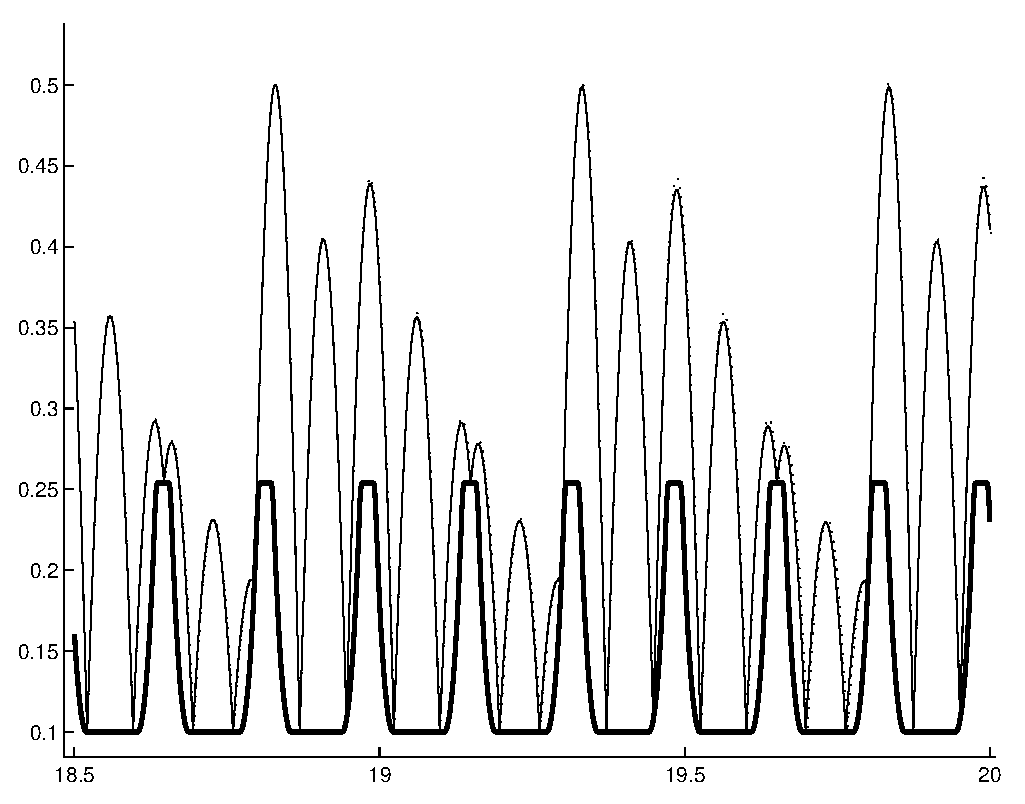
\includegraphics[height=6cm]{./comparison_figs/time_comparison_358}}}
  \put (35,-4){\mbox{\textit{(a)}}}
\end{picture}
\begin{picture}(60,60)(15,-7)
 \put (0,0){\mbox{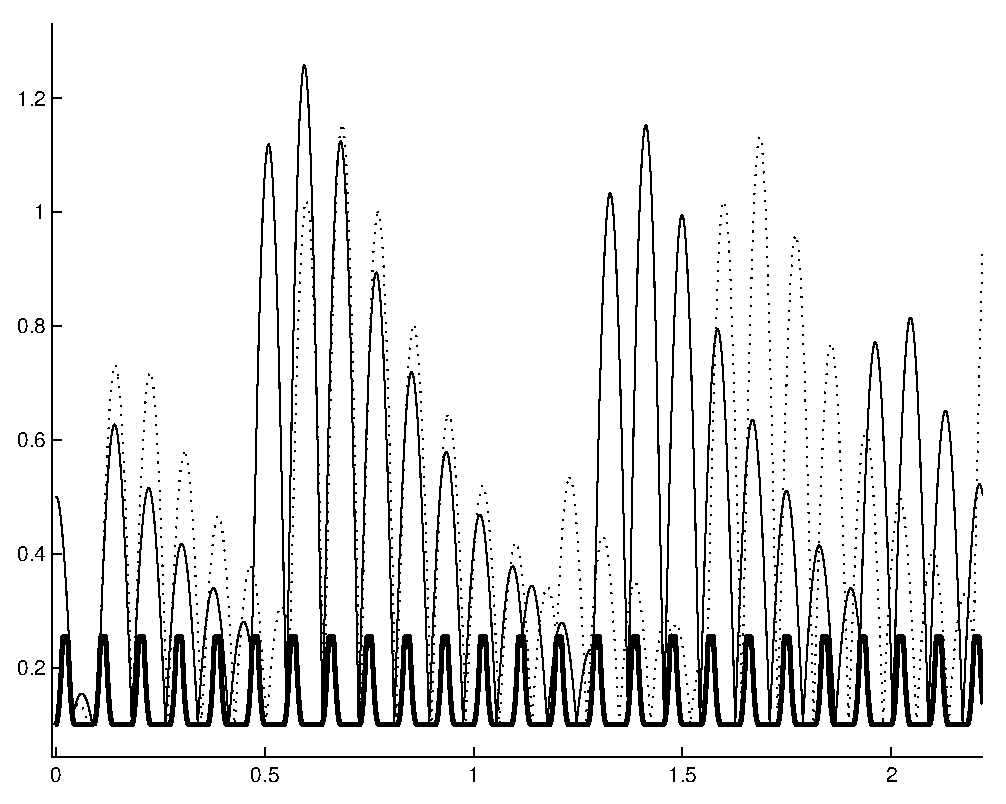
\includegraphics[height=6cm]{./comparison_figs/time_comparison_660}}}
 \put (35,-4){\mbox{\textit{(b)}}}
\end{picture}
\begin{picture}(60,60)(-40,-2)
 \put (0,0){\mbox{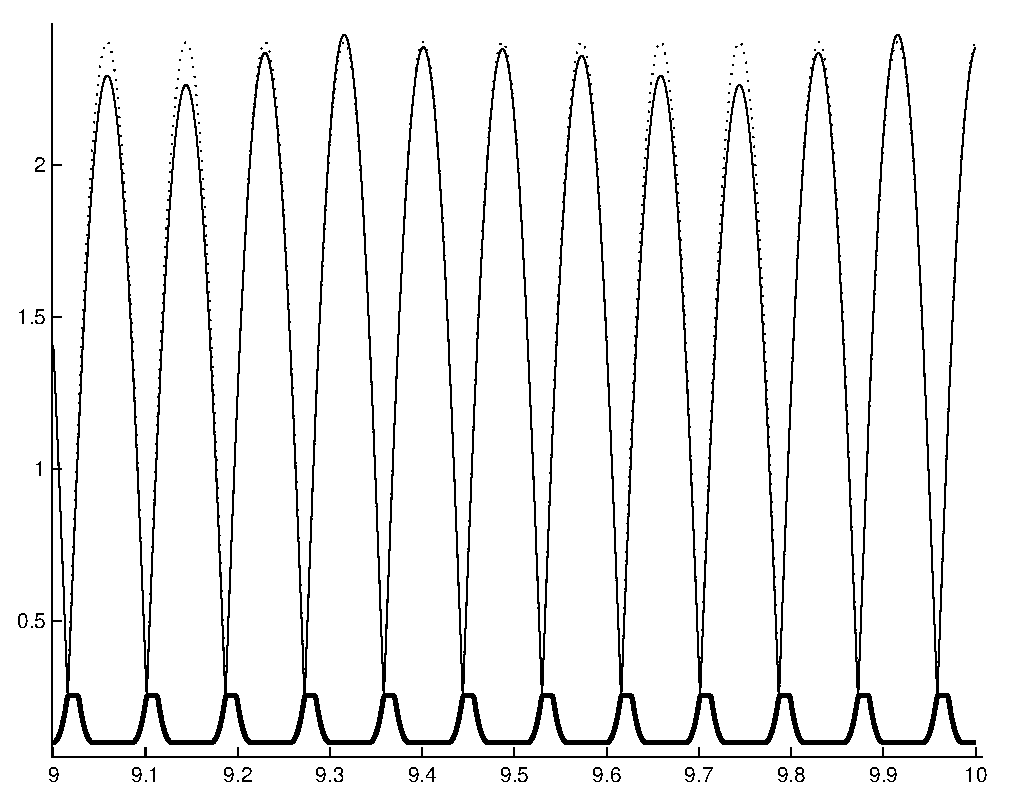
\includegraphics[height=6cm]{./comparison_figs/time_comparison_700}}}
 \put (35,-4){\mbox{\textit{(c)}}}
\end{picture}
  \caption{Time series using SICONOS platform. Time-stepping scheme (continuous line). Event-driven scheme (dashed line) \textit{(a)} rpm=358. \textit{(b)} rpm=660. \textit{(c)} rpm=700.}
  \label{Fig:time_comparison}
\end{figure}

\begin{figure}[hbtp]
\vspace{5mm} \setlength{\unitlength}{1mm}
\begin{picture}(60,60)(0,-7)
 \put (0,0){\mbox{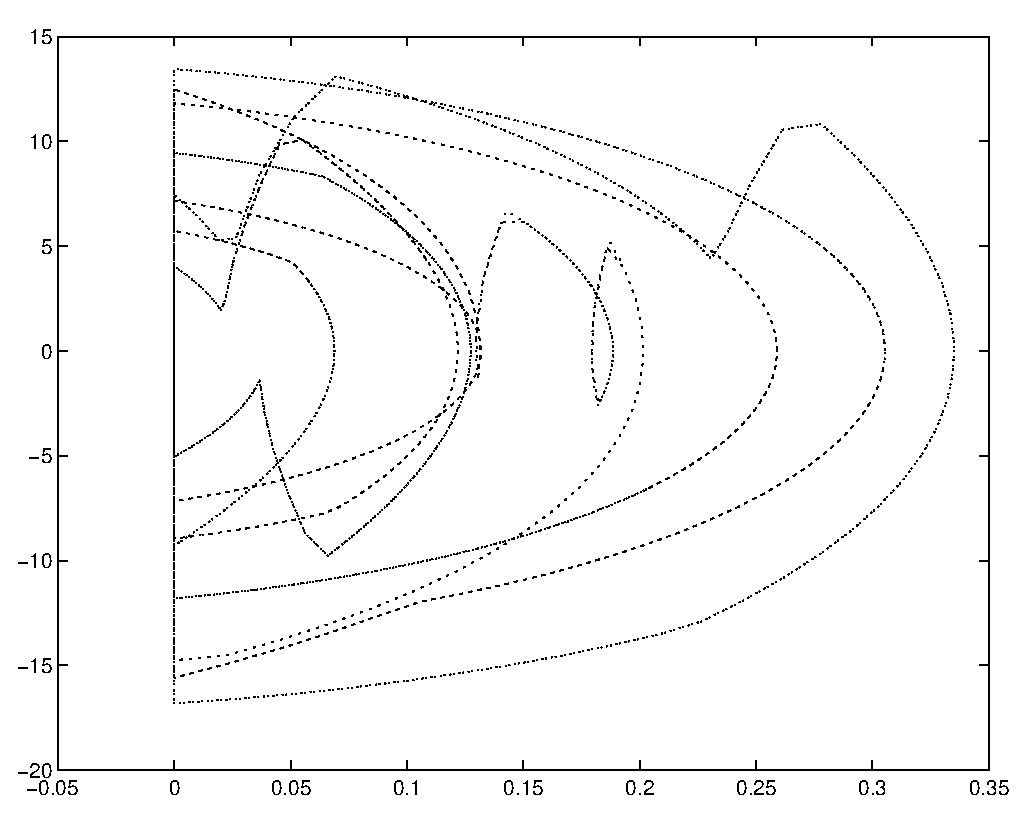
\includegraphics[height=6cm]{./comparison_figs/state_comparison_358event}}}
  \put (35,-4){\mbox{\textit{(a)}}}
\end{picture}
\begin{picture}(60,60)(15,-7)
 \put (0,0){\mbox{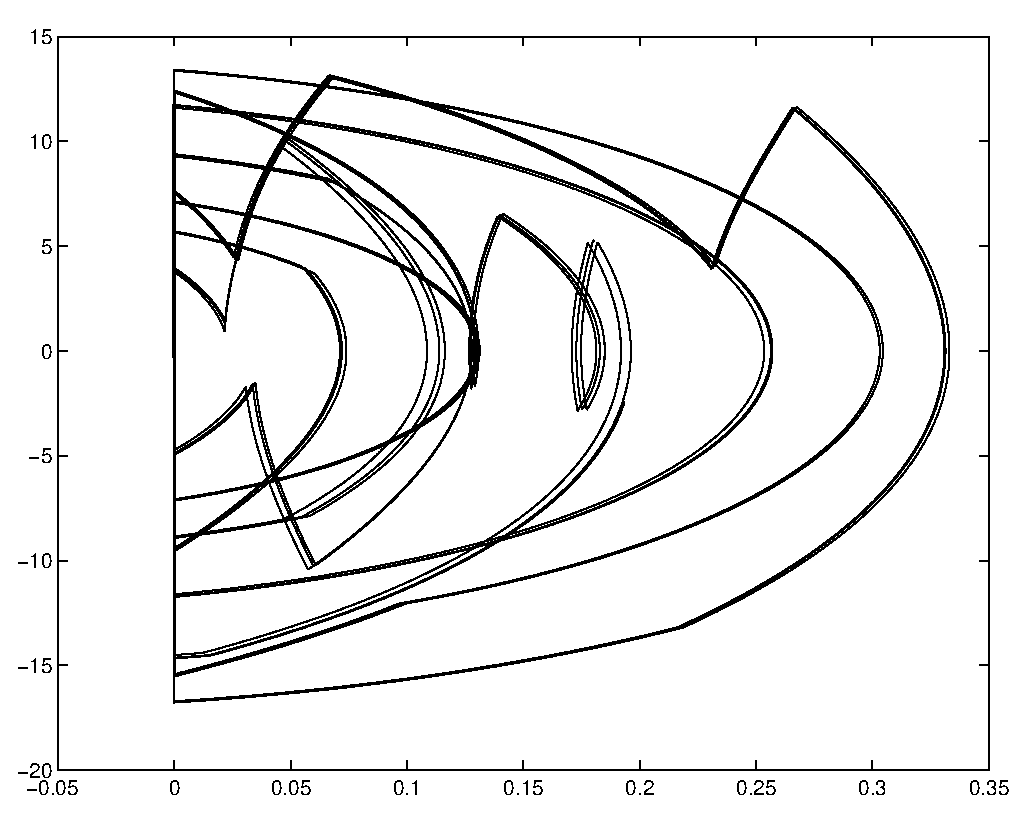
\includegraphics[height=6cm]{./comparison_figs/state_comparison_358siconos}}}
 \put (35,-4){\mbox{\textit{(b)}}}
\end{picture}
\begin{picture}(60,60)(0,-2)
 \put (0,0){\mbox{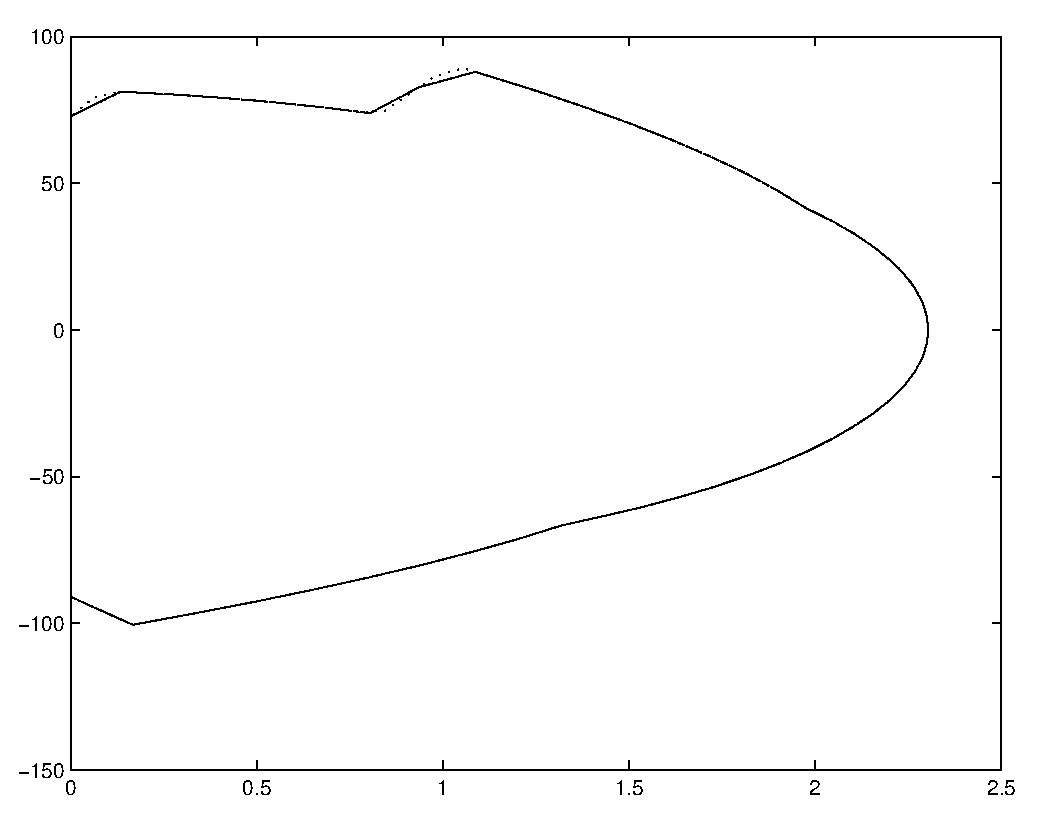
\includegraphics[height=6cm]{./comparison_figs/state_comparison_700event}}}
  \put (35,-4){\mbox{\textit{(c)}}}
\end{picture}
\begin{picture}(60,60)(-17,-2)
 \put (0,0){\mbox{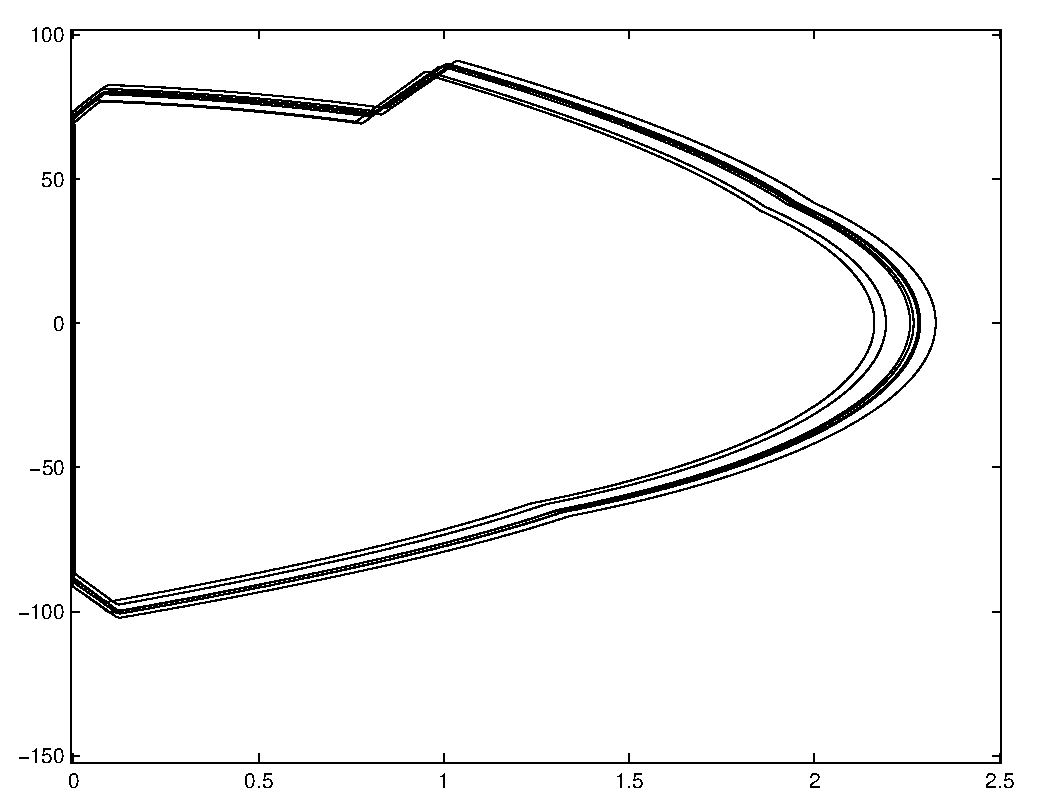
\includegraphics[height=6cm]{./comparison_figs/state_comparison_700siconos}}}
 \put (35,-4){\mbox{\textit{(d)}}}
\end{picture}
  \caption{State space comparison using SICONOS platform. \textit{(a)} rpm=358. Event Driven \textit{(b)} rpm=358. Time Stepping ($h=1e^{-4}$)\textit{(c)} rpm=700. Event Driven \textit{(d)} rpm=700. Time Stepping ($h=1e^{-4}$)}
  \label{Fig:state_comparison}
\end{figure}

\begin{figure}[hbtp]
\vspace{5mm} \setlength{\unitlength}{1mm}
\begin{picture}(60,60)(0,-7)
 \put (0,0){\mbox{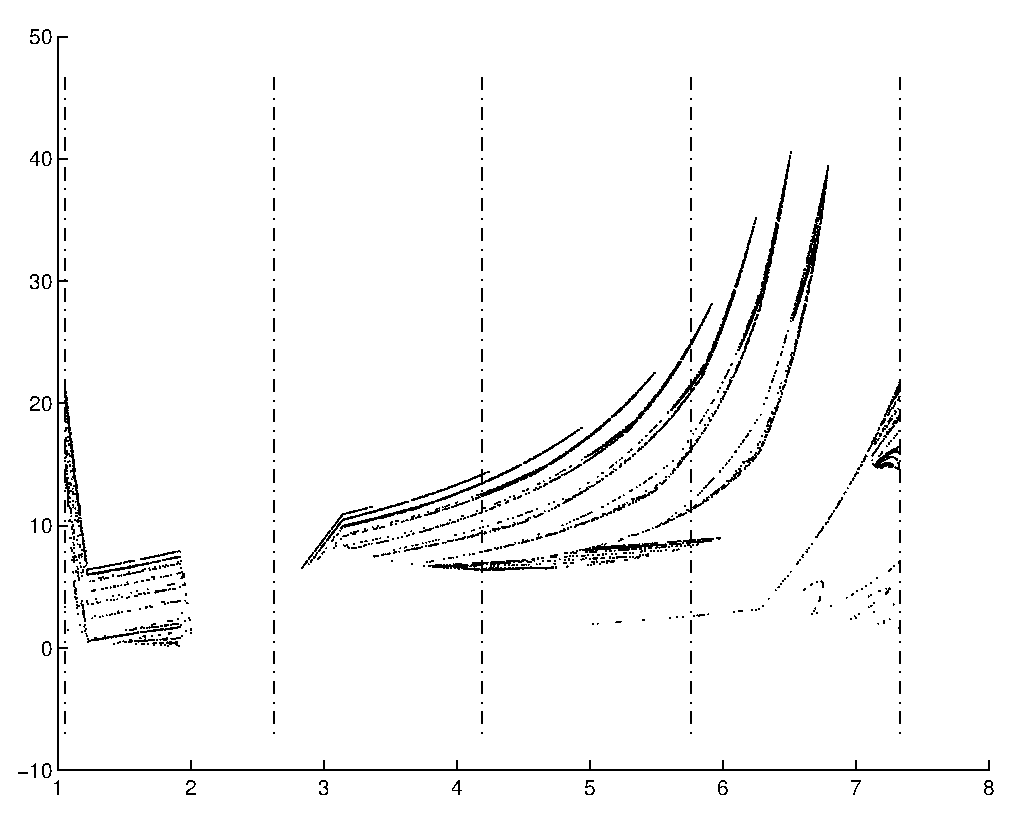
\includegraphics[height=6cm]{./comparison_figs/impact_map_660event}}}
  \put (35,-4){\mbox{\textit{(a)}}}
\end{picture}
\begin{picture}(60,60)(15,-7)
 \put (0,0){\mbox{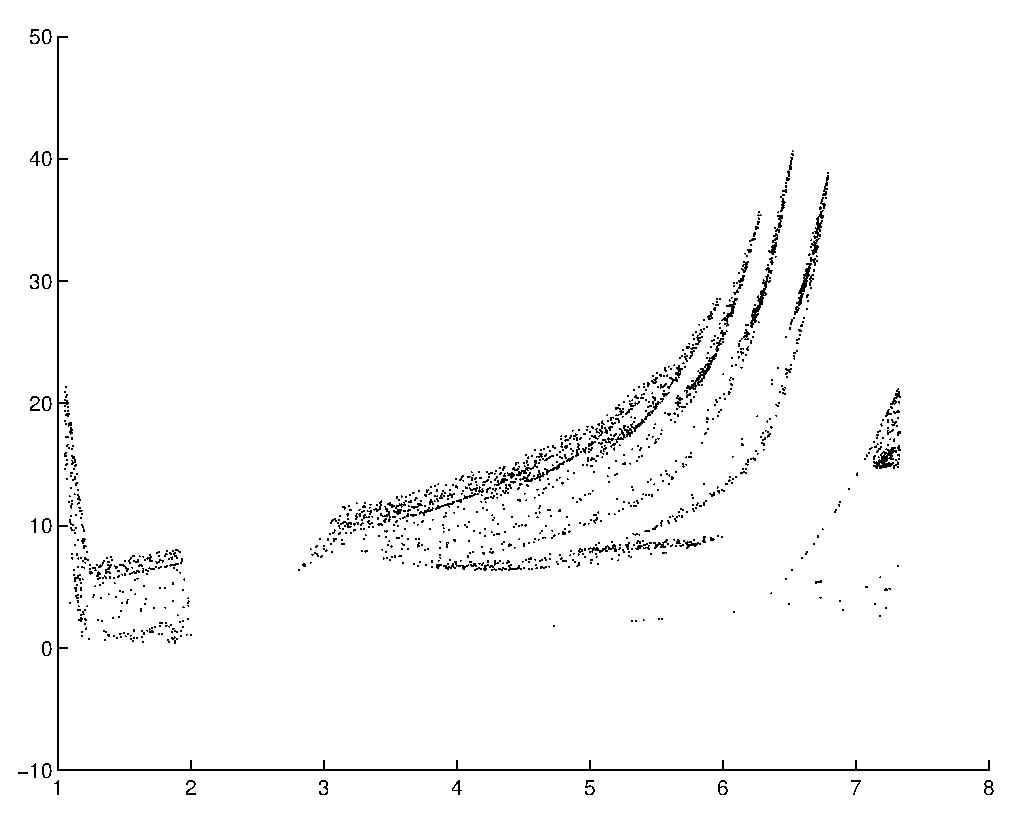
\includegraphics[height=6cm]{./comparison_figs/impact_map_660siconos}}}
 \put (35,-4){\mbox{\textit{(b)}}}
\end{picture}
\begin{picture}(60,60)(0,-2)
 \put (0,0){\mbox{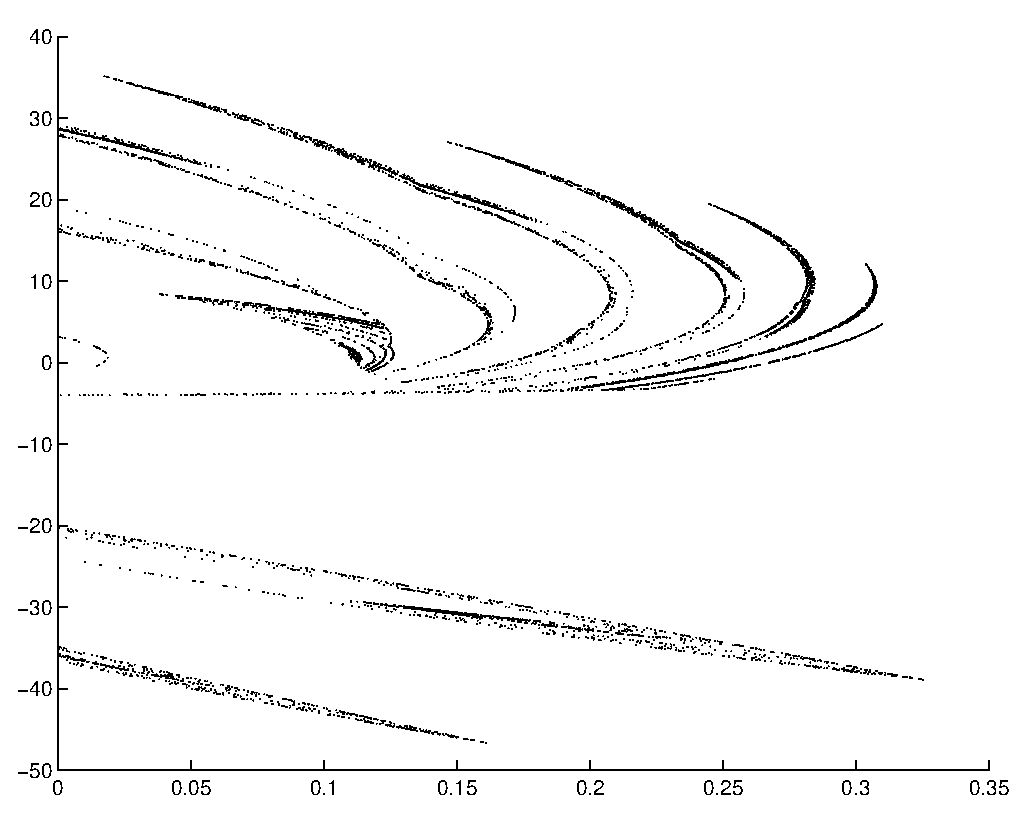
\includegraphics[height=6cm]{./comparison_figs/stroboscopic_map_660event}}}
  \put (35,-4){\mbox{\textit{(c)}}}
\end{picture}
\begin{picture}(60,60)(-17,-2)
 \put (0,0){\mbox{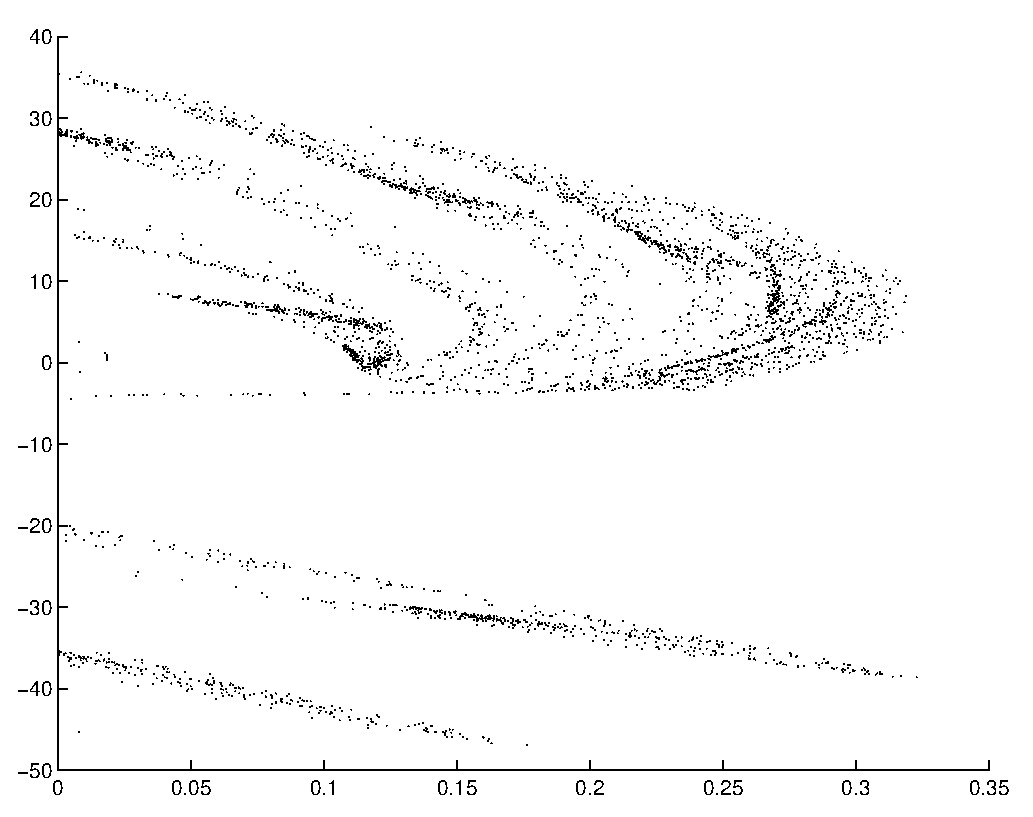
\includegraphics[height=6cm]{./comparison_figs/stroboscopic_map_660siconos}}}
 \put (35,-4){\mbox{\textit{(d)}}}
\end{picture}
  \caption{Attractors comparison using SICONOS platform at rpm=660. \textit{(a)}  Impact map. (Event Driven) \textit{(b)} Impact Map. Time Stepping ($h=1e^{-4}$)\textit{(a)}  Stroboscopic map. (Event Driven) \textit{(b)} Stroboscopic Map. Time Stepping ($h=1e^{-4}$)}
  \label{Fig:attractor_comparison}
\end{figure}

\end{document}
